\documentclass[11pt]{beamer}

%%%%%%%% tema e cor %%%%%%%%
\mode<presentation> {
\usetheme{Madrid}
%\usecolortheme{albatross}
}

\usepackage[utf8]{inputenc}
\usepackage{graphicx} 
\usepackage{booktabs} 
\usepackage[options ]{algorithm2e}

\date{\today}

\AtBeginSection[]
{
\begin{frame}
\frametitle{Curriculum Plan}
\tableofcontents[currentsection]
\end{frame}
}

%%%%%%%% titulo e subtitulo %%%%%%%%
\title[AI4ALL Computer Vision]{Image feature extraction}

\subtitle{(shallow and deep)}

%%%%%%%% nome dos autores %%%%%%%%
\author[Andrew Kondrich]{Andrew Kondrich} 

\begin{document}
\begin{frame}
\titlepage 

\end{frame}

\begin{frame}
\frametitle{Class schedule} 
\tableofcontents 
\end{frame}

%%%%%%%% slides %%%%%%%%
\section{Recap: Image Representation}
\begin{frame}{Image Representation}
\begin{figure}
    \centering
    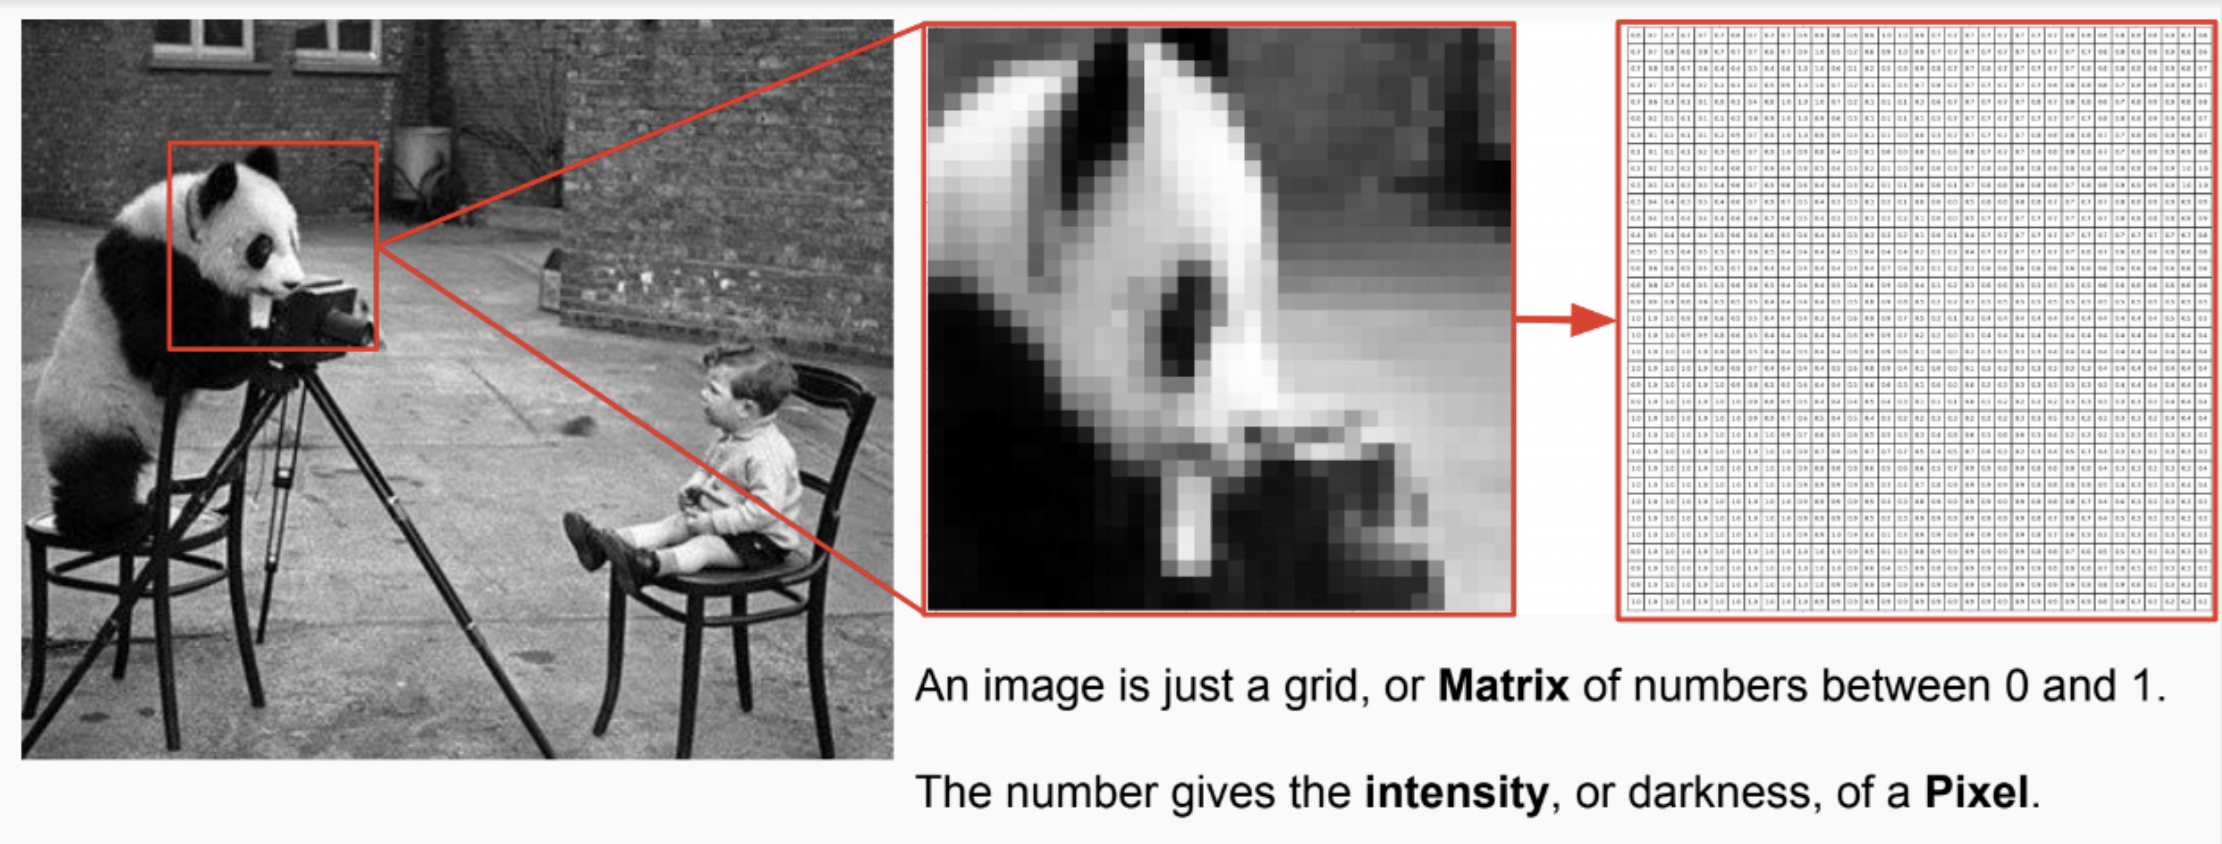
\includegraphics[width=0.9\textwidth]{img/greyscaleimage.png}
    \caption{Black \& White image of panda is a matrix}
\end{figure}
\end{frame}

\begin{frame}{Representing Color}
\begin{figure}
    \centering
    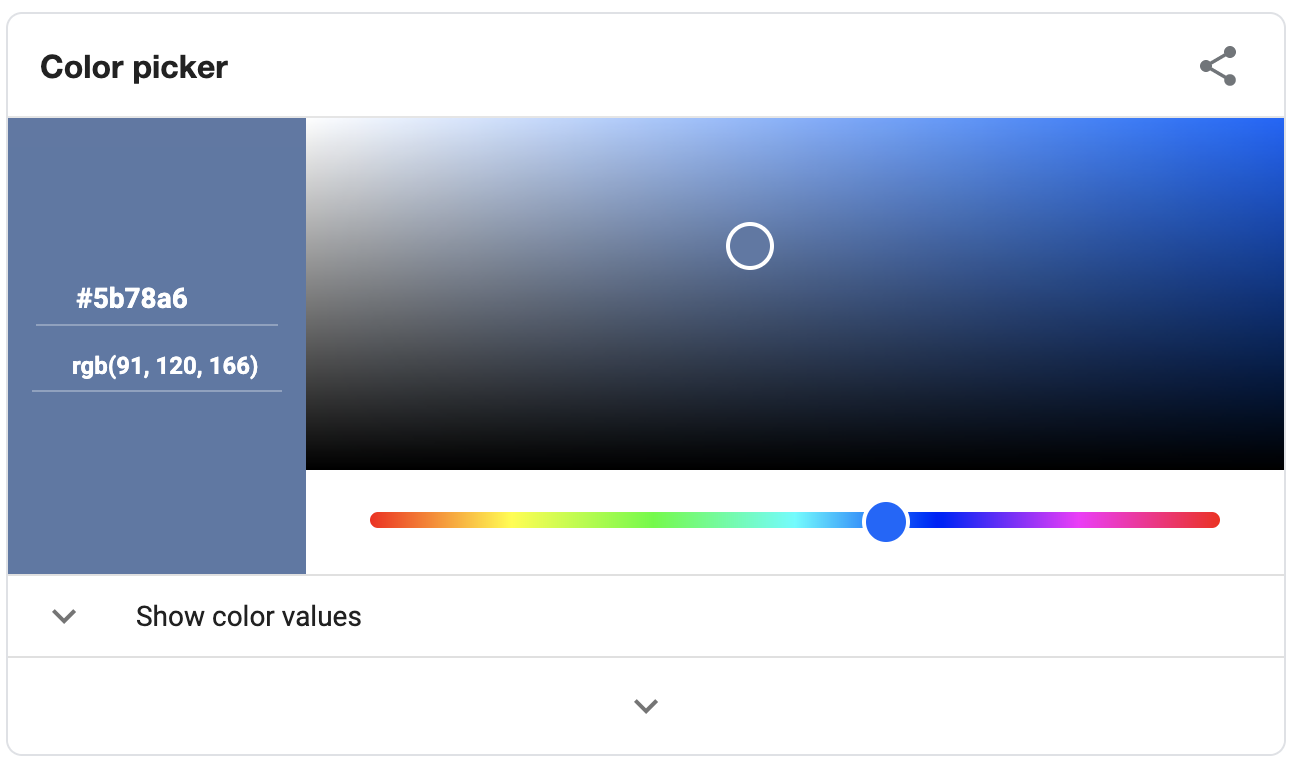
\includegraphics[width=0.9\textwidth]{img/colorpicker.png}
    \caption{Color of single pixel is represented by combination of 3 RGB values}
\end{figure}
\end{frame}

\begin{frame}{Representing Color}
\begin{figure}
    \centering
    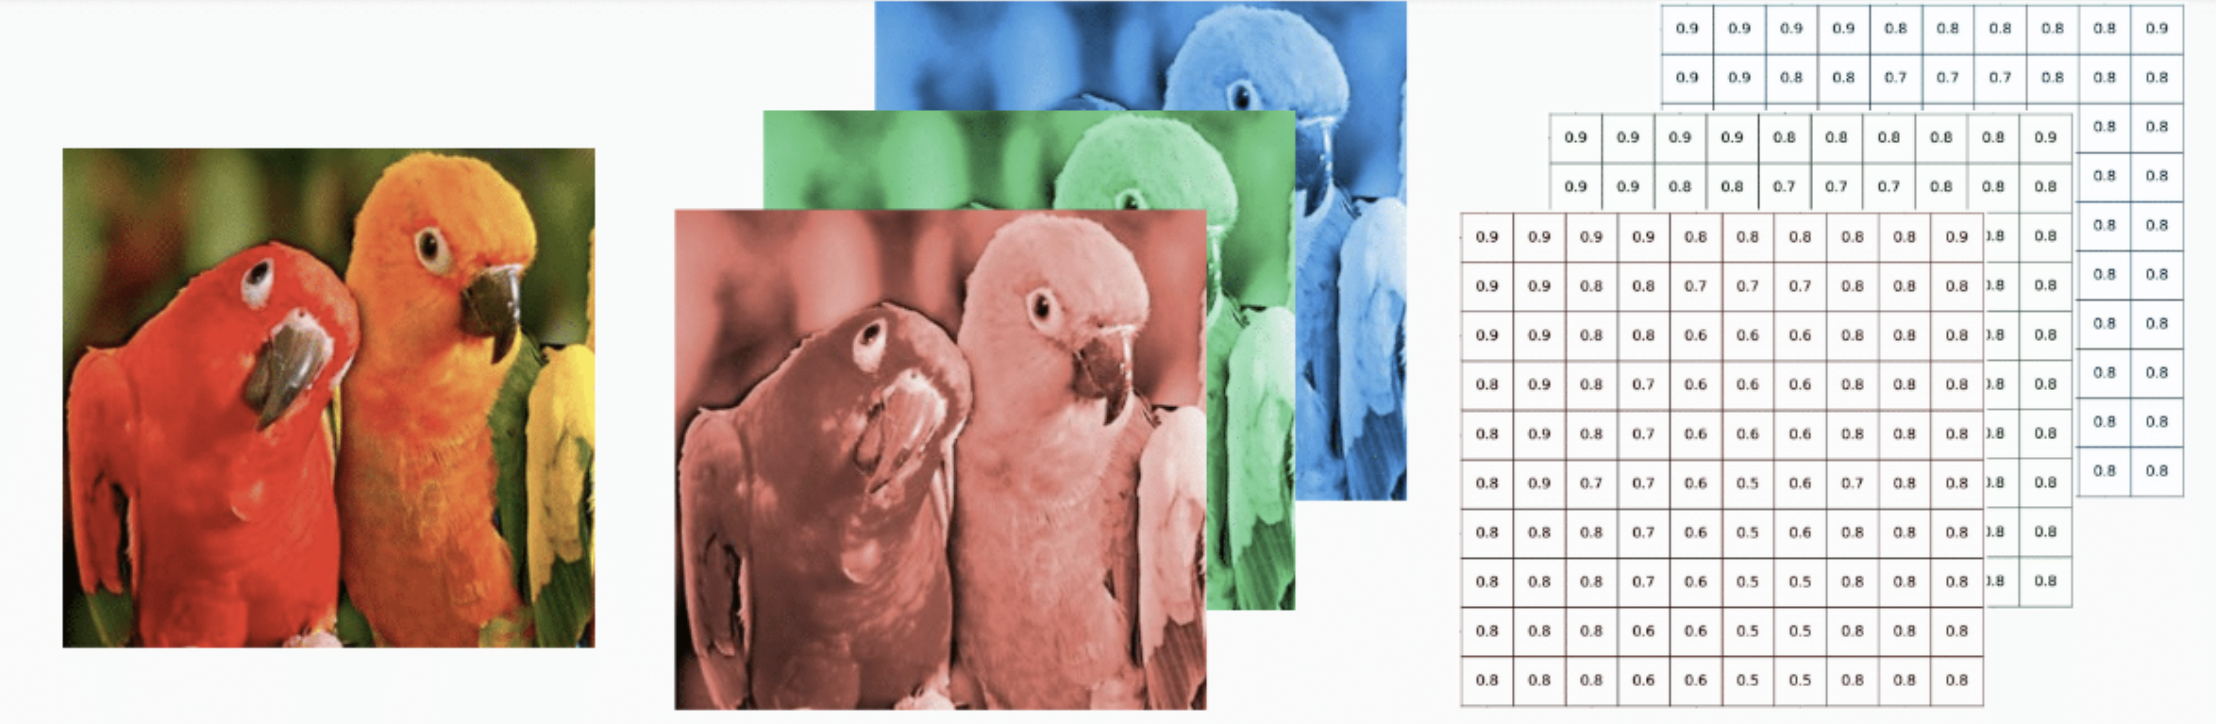
\includegraphics[width=0.9\textwidth]{img/rgbparrot.png}
    \caption{Stacking RGB layers forms final picture}
\end{figure}
\end{frame}

\begin{frame}{Representing Color}
\begin{figure}
    \centering
    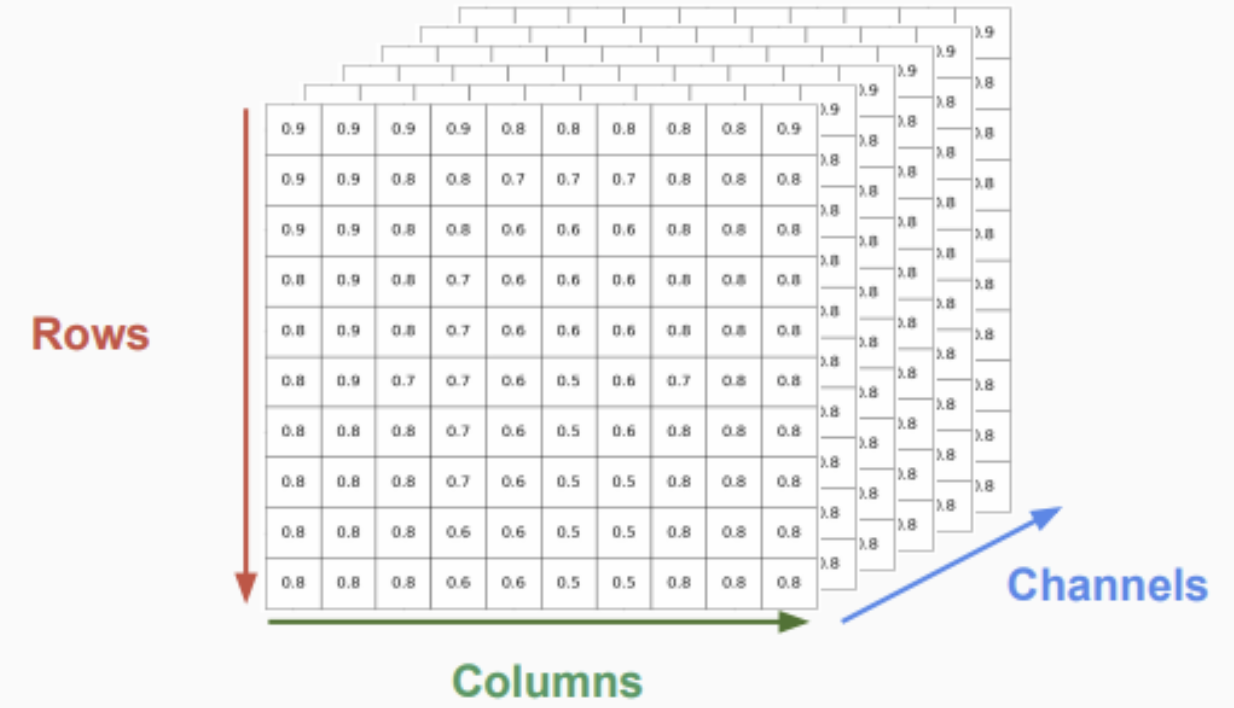
\includegraphics[width=0.7\textwidth]{img/rowcolchannel.png}
    \caption{Numerically, images are 3-dimensional matrices with rows, columns, and 3 \textbf{channels}. We also call these \textbf{volumes}.}
\end{figure}
\end{frame}

\section{Recap: Challenges of Computer Vision}
\begin{frame}{Challenges of Computer Vision}
\begin{itemize}
    \item Because images are very high-dimensional data, it is difficult for models to capture all possible variety and edge cases included in your data.
    \item Example: When using logistic regression, what happens when you shift an entire image left by one pixel?
\end{itemize}
\end{frame}

\begin{frame}{Challenges of Computer Vision}
\begin{figure}
    \centering
    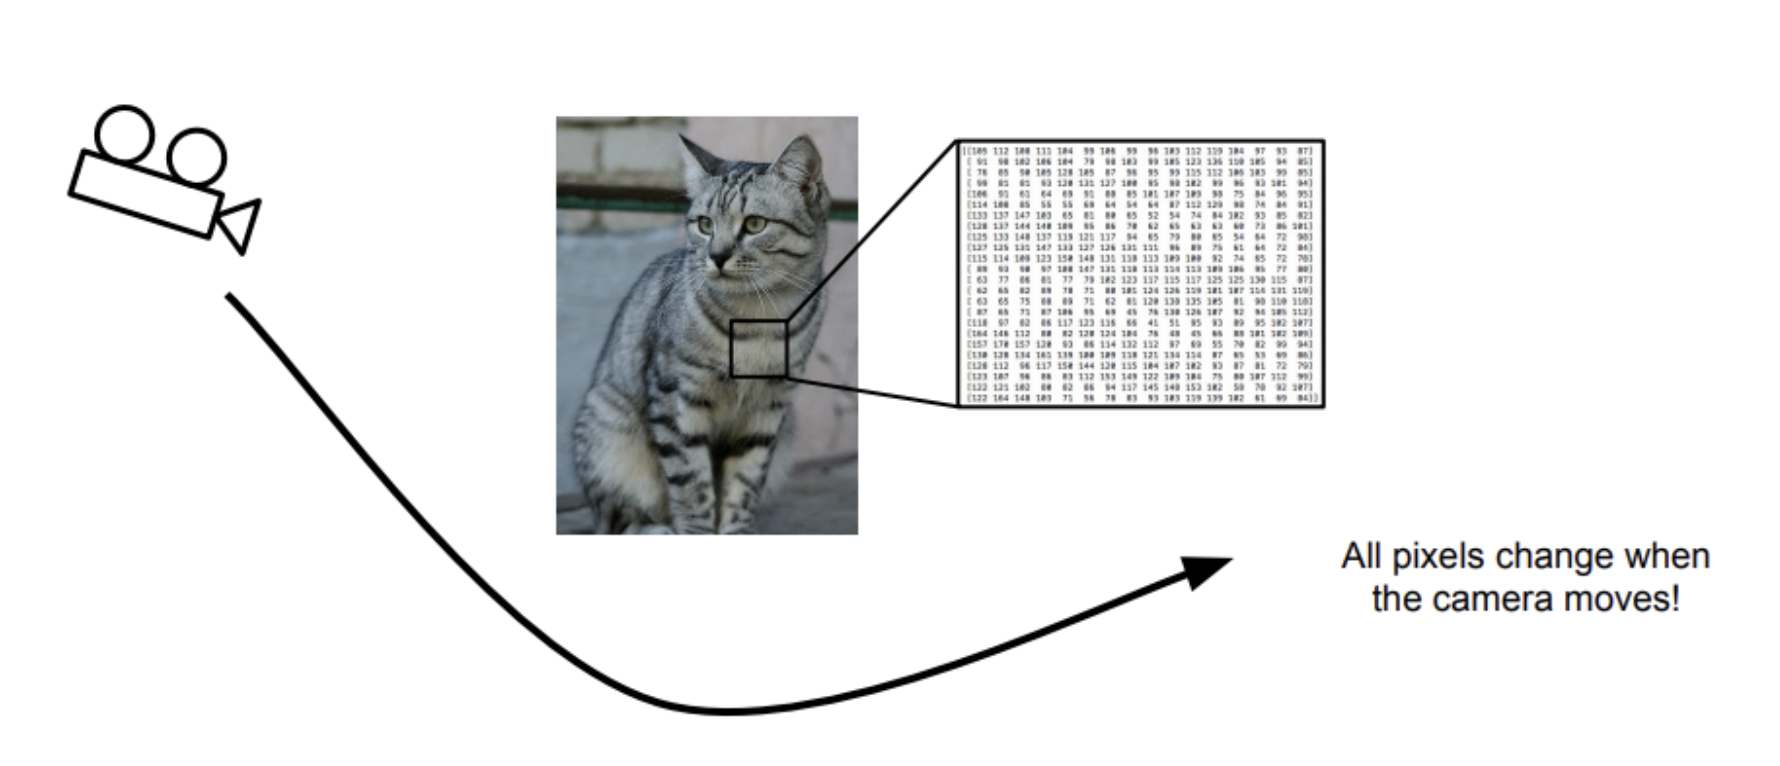
\includegraphics[width=0.9\textwidth]{img/viewpointvariation.png}
    \caption{Viewpoint Variation}
\end{figure}
\footnotetext{http://cs231n.stanford.edu/slides/2019/cs231n\_2019\_lecture02.pdf}
\end{frame}

\begin{frame}{Challenges of Computer Vision}
\begin{figure}
    \centering
    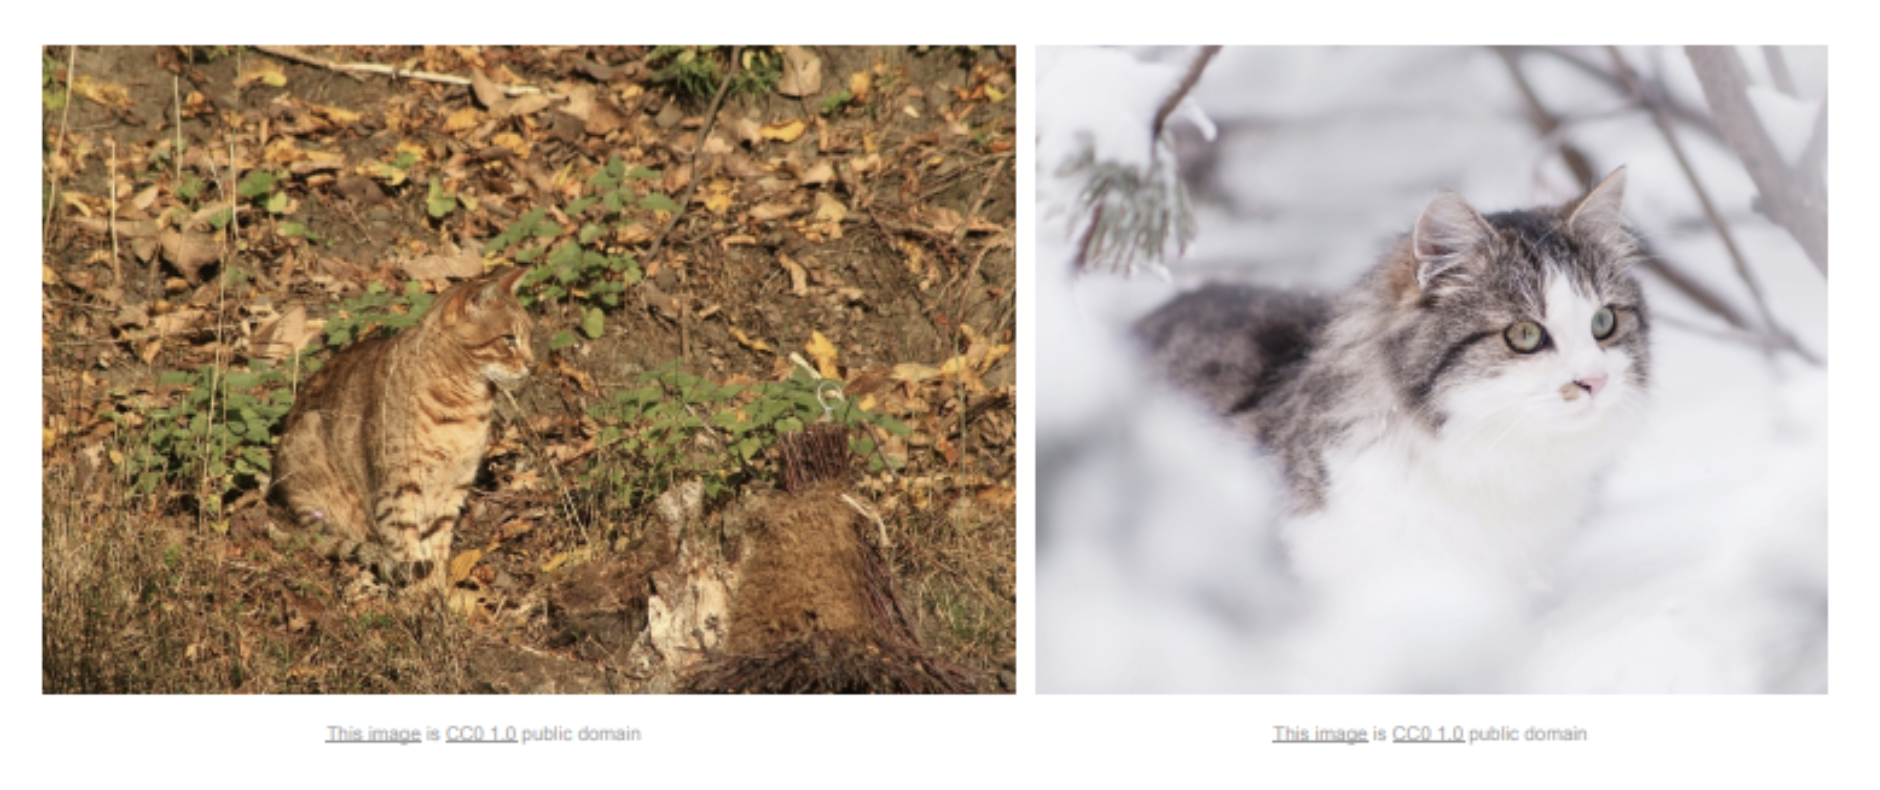
\includegraphics[width=0.9\textwidth]{img/occlusion.png}
    \caption{Background Clutter}
\end{figure}
\footnotetext{http://cs231n.stanford.edu/slides/2019/cs231n\_2019\_lecture02.pdf}
\end{frame}

\begin{frame}{Challenges of Computer Vision}
\begin{figure}
    \centering
    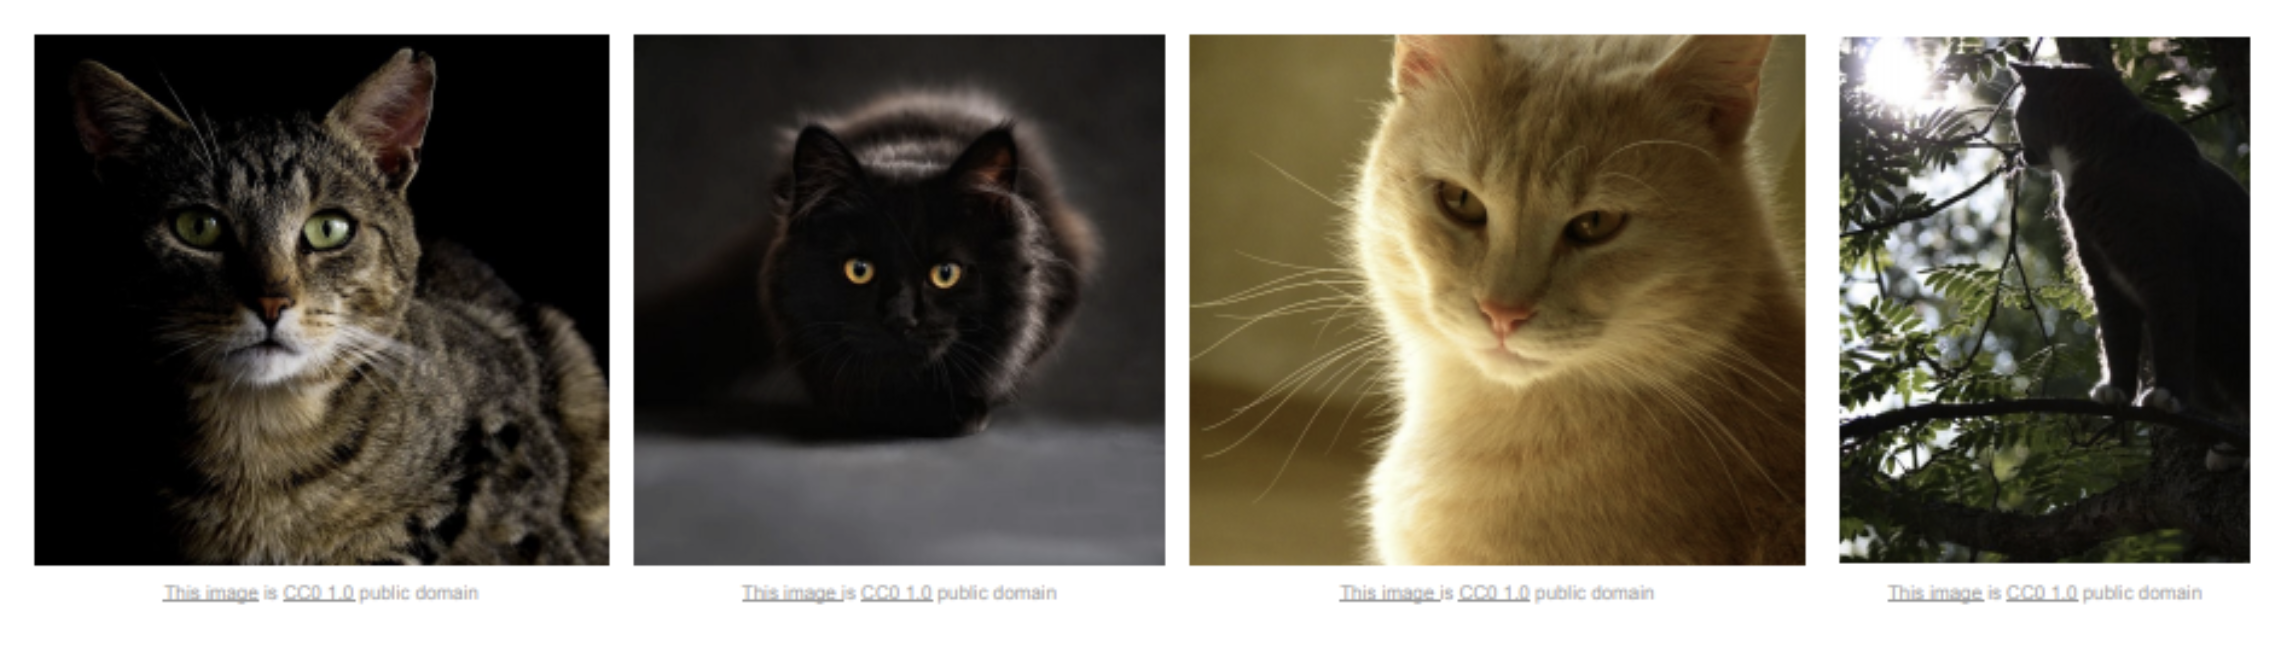
\includegraphics[width=0.9\textwidth]{img/illumination.png}
    \caption{Illumination}
\end{figure}
\footnotetext{http://cs231n.stanford.edu/slides/2019/cs231n\_2019\_lecture02.pdf}
\end{frame}

\begin{frame}{Challenges of Computer Vision}
\begin{figure}
    \centering
    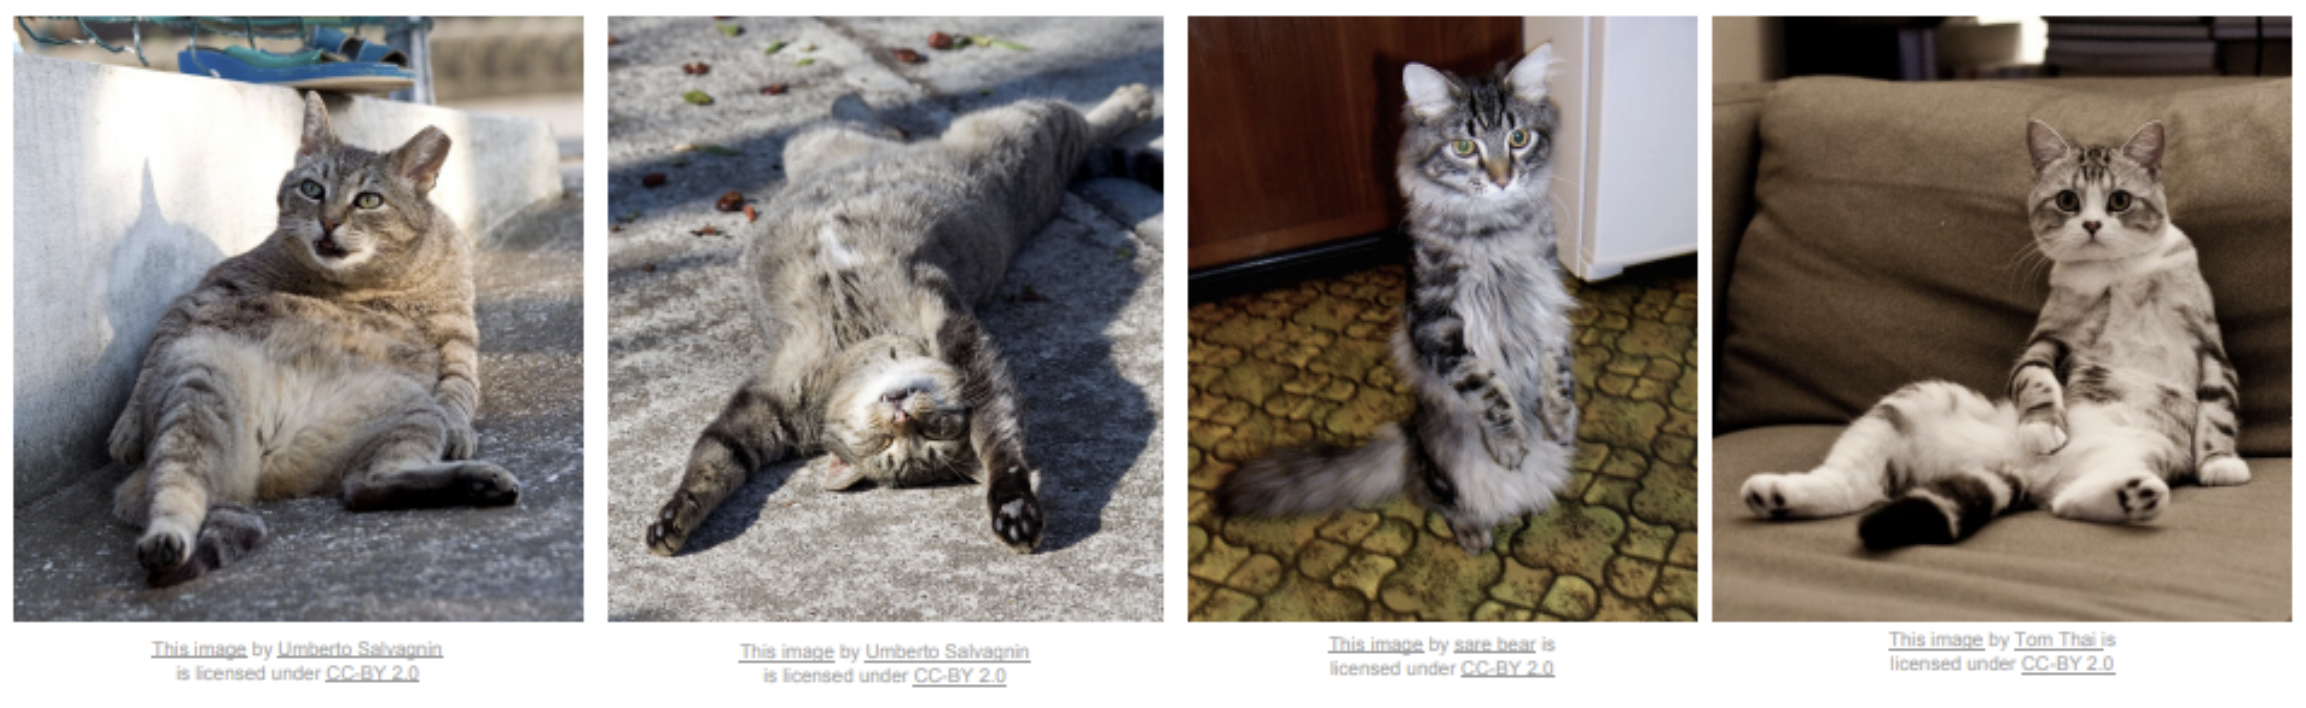
\includegraphics[width=0.9\textwidth]{img/deformation.png}
    \caption{Deformation}
\end{figure}
\footnotetext{http://cs231n.stanford.edu/slides/2019/cs231n\_2019\_lecture02.pdf}
\end{frame}

\begin{frame}{Challenges of Computer Vision}
\begin{figure}
    \centering
    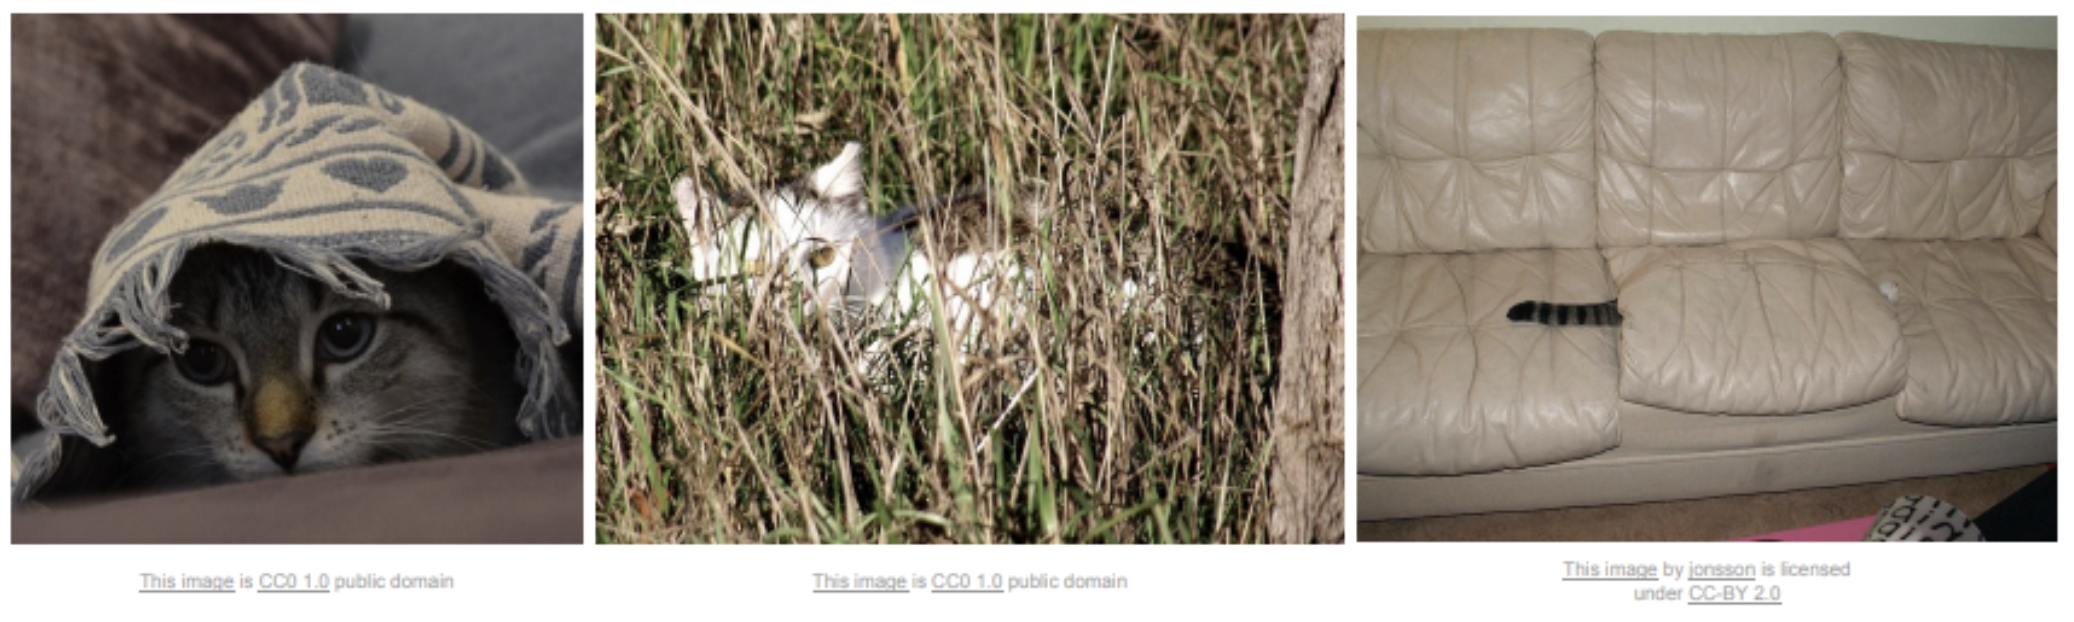
\includegraphics[width=0.9\textwidth]{img/hiding.png}
    \caption{Occlusion}
\end{figure}
\footnotetext{http://cs231n.stanford.edu/slides/2019/cs231n\_2019\_lecture02.pdf}
\end{frame}

\section{Recap: Neural Networks}
\begin{frame}{Neural Networks}
\begin{figure}
    \centering
    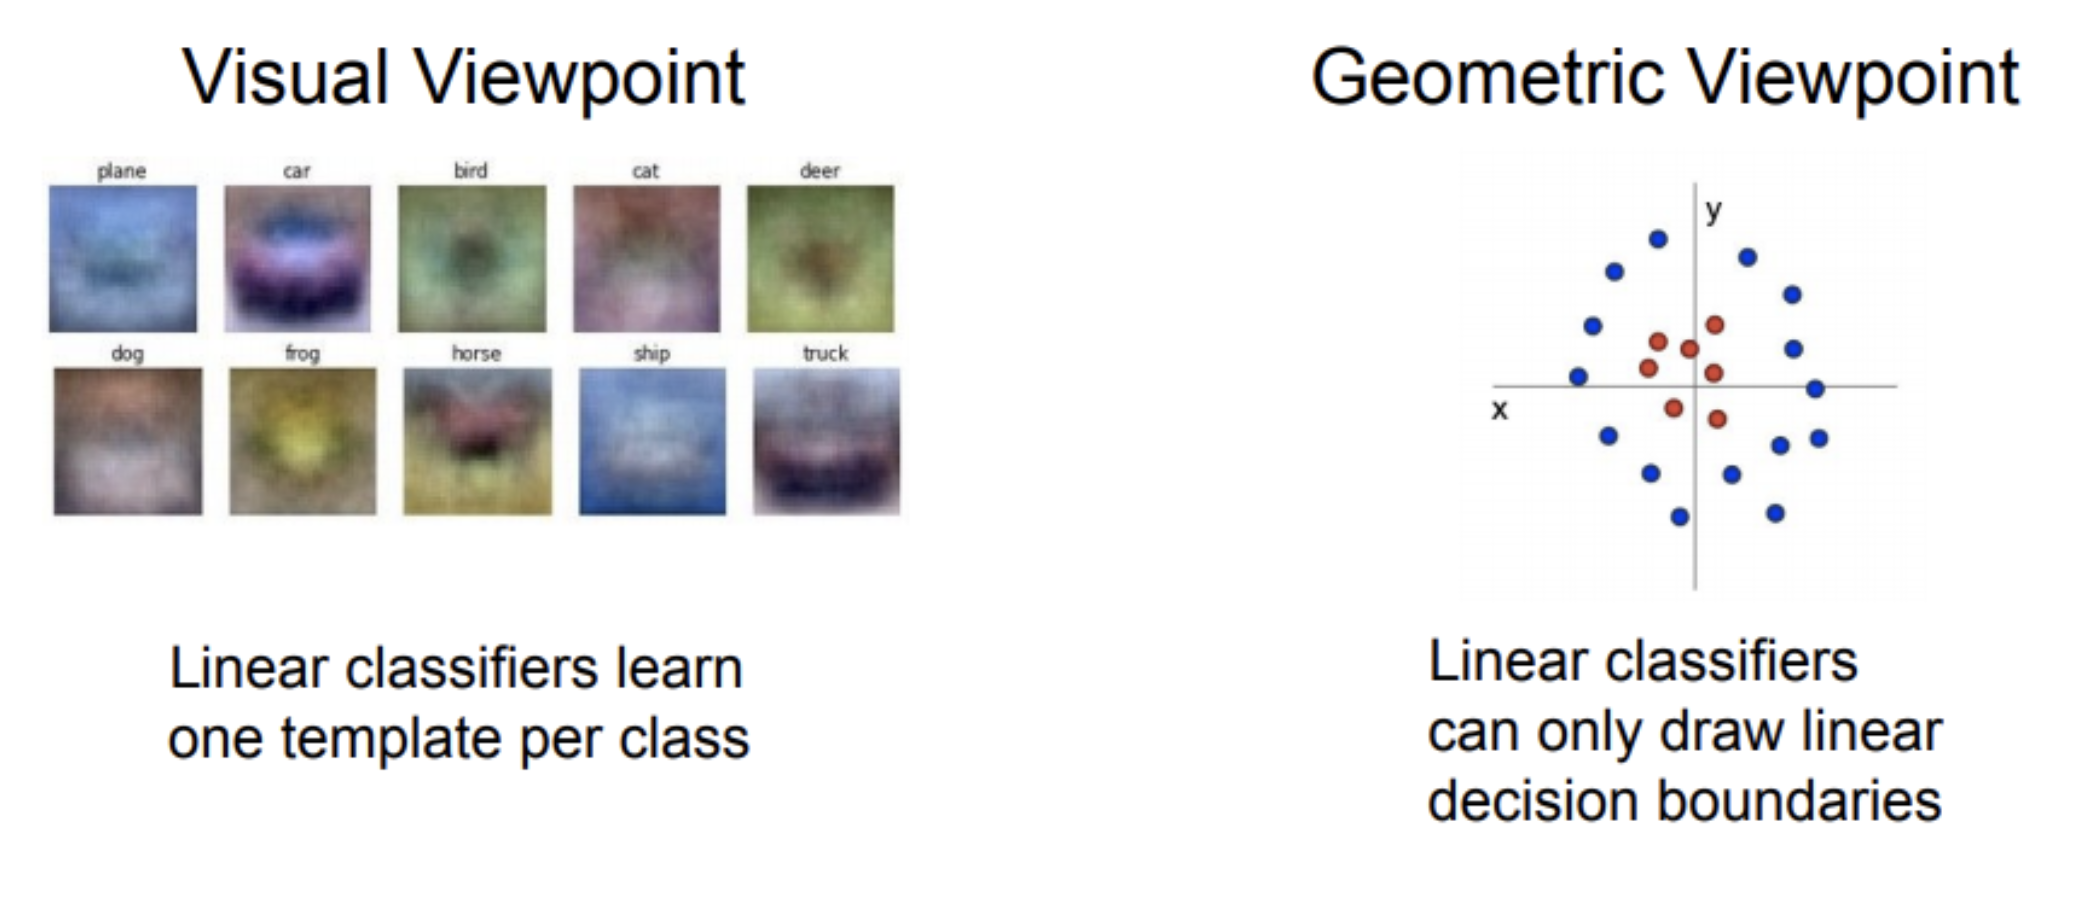
\includegraphics[width=\textwidth]{img/linearweak.png}
    \caption{Motivation: Linear models are fairly weak}
\end{figure}
\footnotetext{http://cs231n.stanford.edu/slides/2019/cs231n\_2019\_lecture02.pdf}
\end{frame}

\begin{frame}{Neural Networks}
\begin{itemize}
    \item We can model more complex functions by "stacking" more weights.
    \item Instead of
    $$\hat{y} = \sigma(\textbf{w} \cdot \textbf{x})$$
    We can now also do this:
    $$\hat{y} = \sigma(\textbf{w}_1 \cdot \sigma(\textbf{w}_2 \cdot \textbf{x}))$$
    $$\textbf{w}_1 \in \mathbf{R}^M, \textbf{w}_2 \in \textbf{R}^{M \times D}, \textbf{x} \in \textbf{R}^D$$
    Each row of the matrix $\textbf{w}_2$ is called a "neuron"
\end{itemize}
\end{frame}

\begin{frame}{Neural Networks}
\begin{figure}
    \centering
    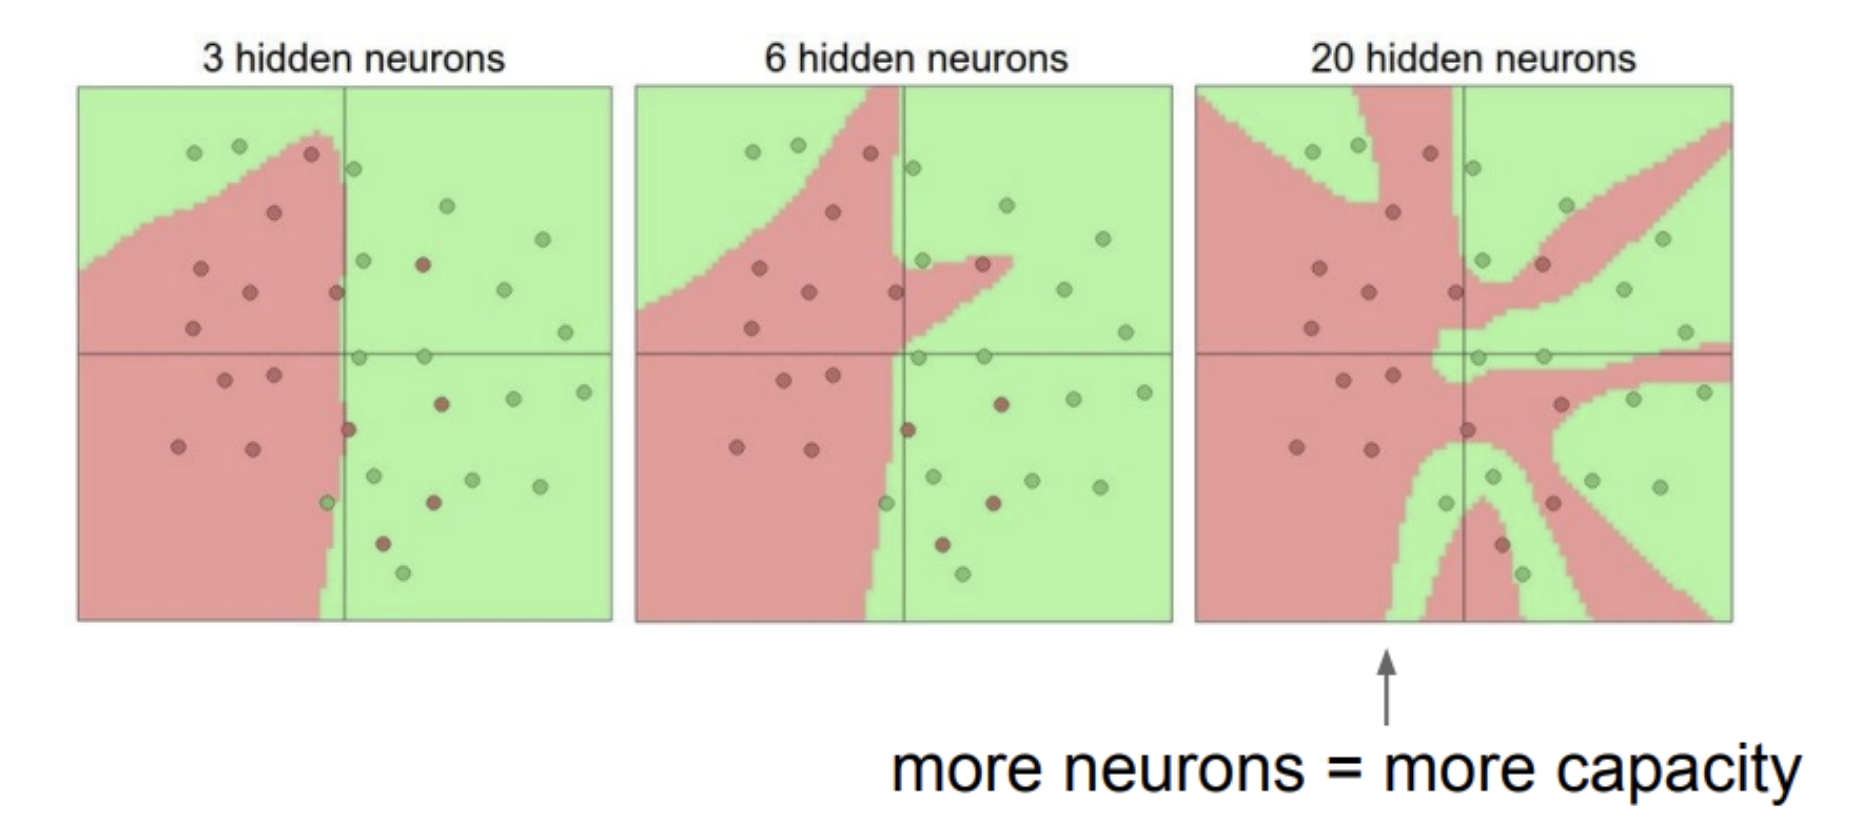
\includegraphics[width=0.8\textwidth]{img/moreneuronmorecap.png}
    \caption{The more neurons you have, the more \textbf{expressive} your model is.}
\end{figure}
\footnotetext{http://cs231n.github.io/neural-networks-1/}
\end{frame}

\begin{frame}{Neural Networks}
\begin{figure}
    \centering
    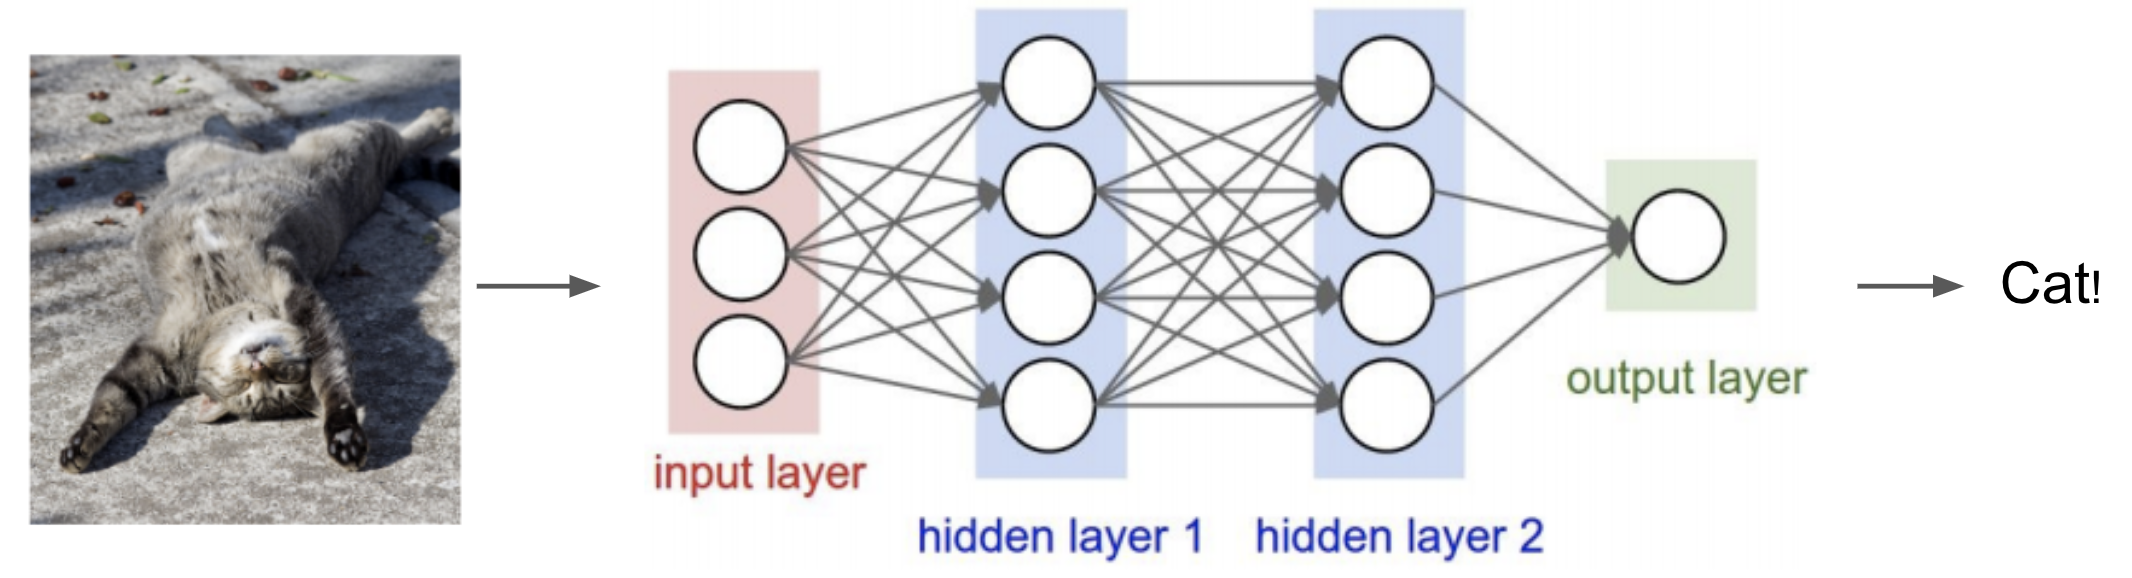
\includegraphics[width=\textwidth]{img/catNN.png}
    \caption{By stacking more and more layers and adding neurons, we can get models capable of representing all cats!}
\end{figure}
\end{frame}

\section{Invariant Local Features}
\begin{frame}{Invariant Local Features}
\begin{figure}
    \centering
    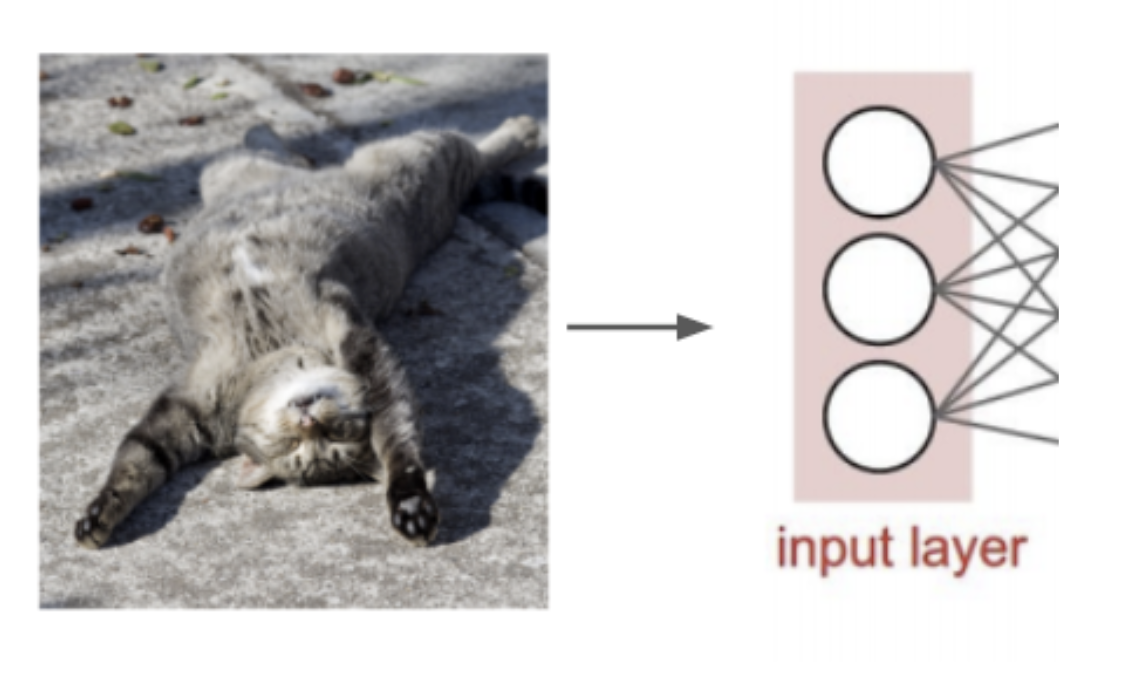
\includegraphics[width=0.9\textwidth]{img/catinput.png}
    \caption{What is the best way to pass an image into a neural network?}
\end{figure}
\end{frame}

\begin{frame}{Invariant Local Features}
\begin{figure}
    \centering
    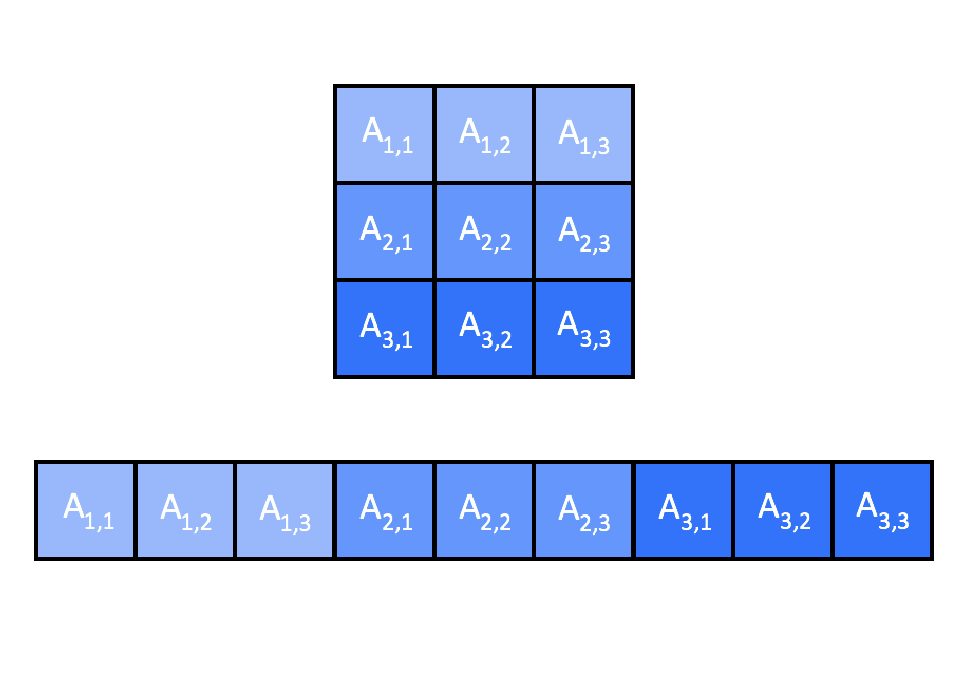
\includegraphics[width=0.7\textwidth]{img/flatten.png}
    \caption{What could be wrong with just flattening images?}
\end{figure}
\end{frame}

\begin{frame}{Invariant Local Features}
What could be wrong with just flattening images?
\begin{itemize}
    \item Images are huge: How many features in a 128x128x3 image?
\end{itemize}
\end{frame}

\begin{frame}{Invariant Local Features}
What could be wrong with just flattening images?
\begin{itemize}
    \item Images are huge: How many features in a 128x128x3 image?
    \item For every change in viewpoint, you would change 49,152 features.
\end{itemize}
\end{frame}

\begin{frame}{Invariant Local Features}
What could be wrong with just flattening images?
\begin{itemize}
    \item Images are huge: How many features in a 128x128x3 image?
    \item For every change in viewpoint, you would change 49,152 features.
    \item You don't take advantage of \textbf{locality}
\end{itemize}
\end{frame}

\begin{frame}{Invariant Local Features}
\begin{figure}
    \centering
    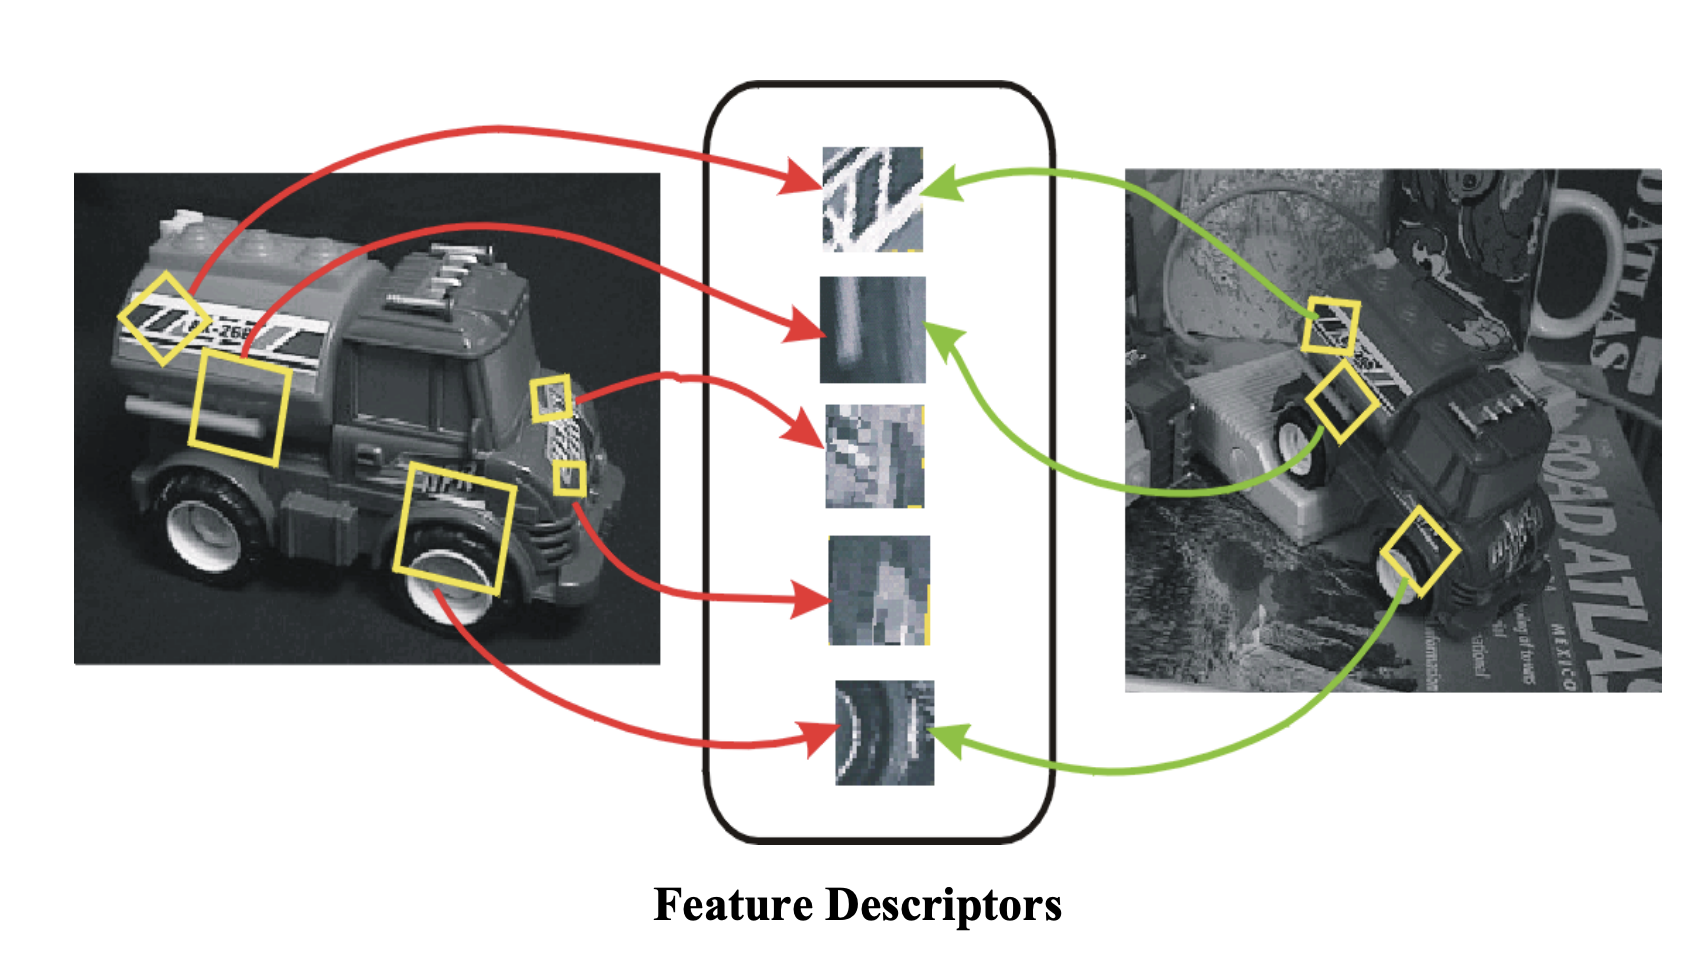
\includegraphics[width=0.7\textwidth]{img/invariantlocal.png}
    \caption{Patterns in images should remain the same even if picture changes}
\end{figure}
[Source: N. Snavely]
\end{frame}

\begin{frame}{Invariant Local Features}
    What are advantages of local features?
    \begin{itemize}
        \item Locality: features are local, so robust to occlusion and clutter
        \item Quantity: hundreds or thousands in a single image
        \item Distinctiveness: can differentiate a large database of objects
    \end{itemize}
\end{frame}

\begin{frame}{Invariant Local Features}
Suppose we only consider a small window of pixels
\begin{itemize}
    \item Look for image regions that are unusual: lead to unambiguous matches in other images
    \item How to define ”unusual”?
\end{itemize}
\end{frame}

\begin{frame}{Invariant Local Features}
Suppose we only consider a small window of pixels
\begin{itemize}
    \item What defines whether a feature is a good or bad candidate?
    \item (This intuition is used in the famous Harris Corner Detector)
\end{itemize}
 \begin{figure}
    \centering
    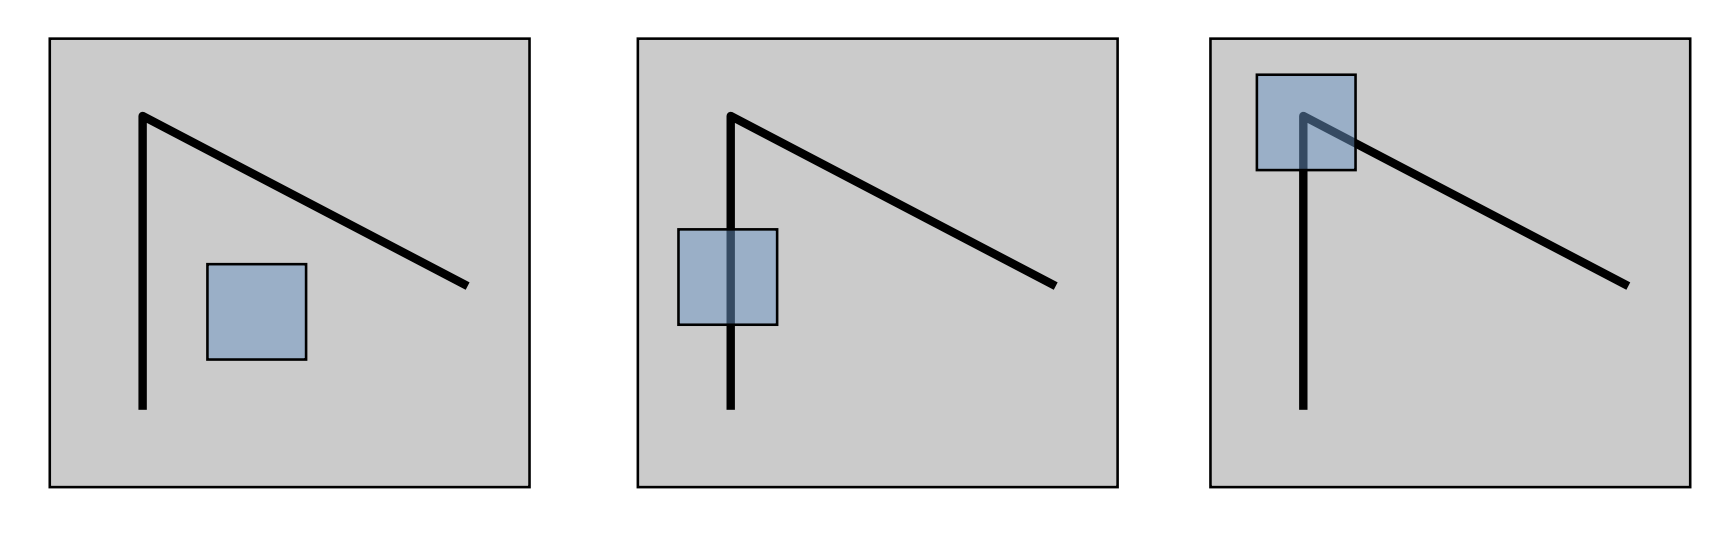
\includegraphics[width=0.7\textwidth]{img/edgebest.png}
    \caption{Which window would change the most if you shift it?}
\end{figure}  
    [Source: S. Seitz, D. Frolova, D. Simakov]

\end{frame}



\section{Classical Feature Extraction}
\begin{frame}{Classical Feature Extraction}
\begin{itemize}
    \item \textbf{Problem:} Our images are too high-dimensional and flattening doesn't take advantage of innate local properties of images.
    \item \textbf{Solution:} Can our images be reduced to a set of features (also named a feature vector).
    \item In "classical" feature extraction, we rely on our human understanding of what a "good" local features is to decide what matters in a picture and what doesn't.
\end{itemize}
\end{frame}

\begin{frame}{Classical Feature Extraction}
    \begin{figure}
    \centering
    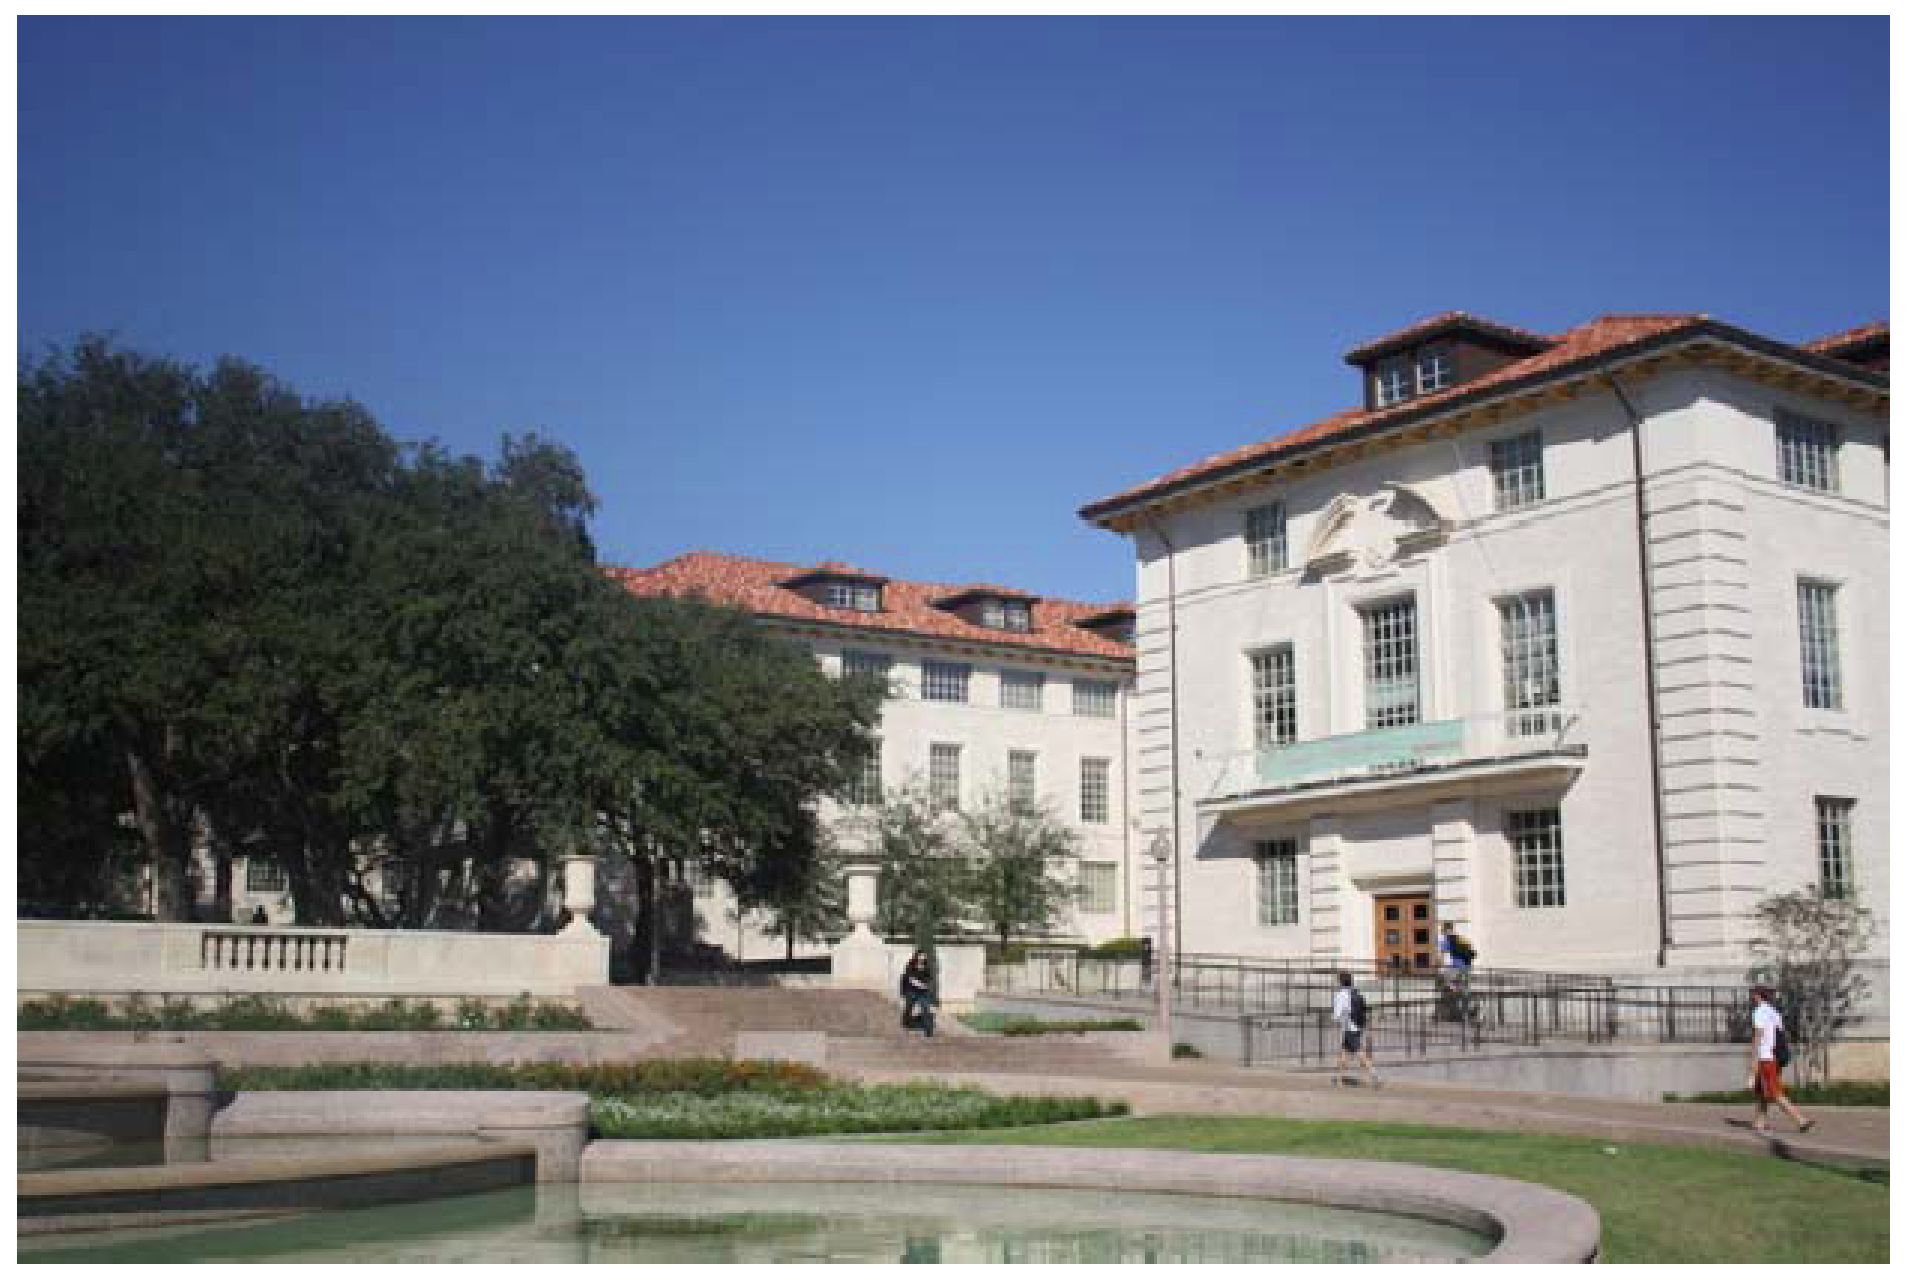
\includegraphics[width=0.8\textwidth]{img/house.png}
    \caption{Standard Image of a campus}
    \end{figure}
\end{frame}

\begin{frame}{Classical Feature Extraction}
    \begin{figure}
    \centering
    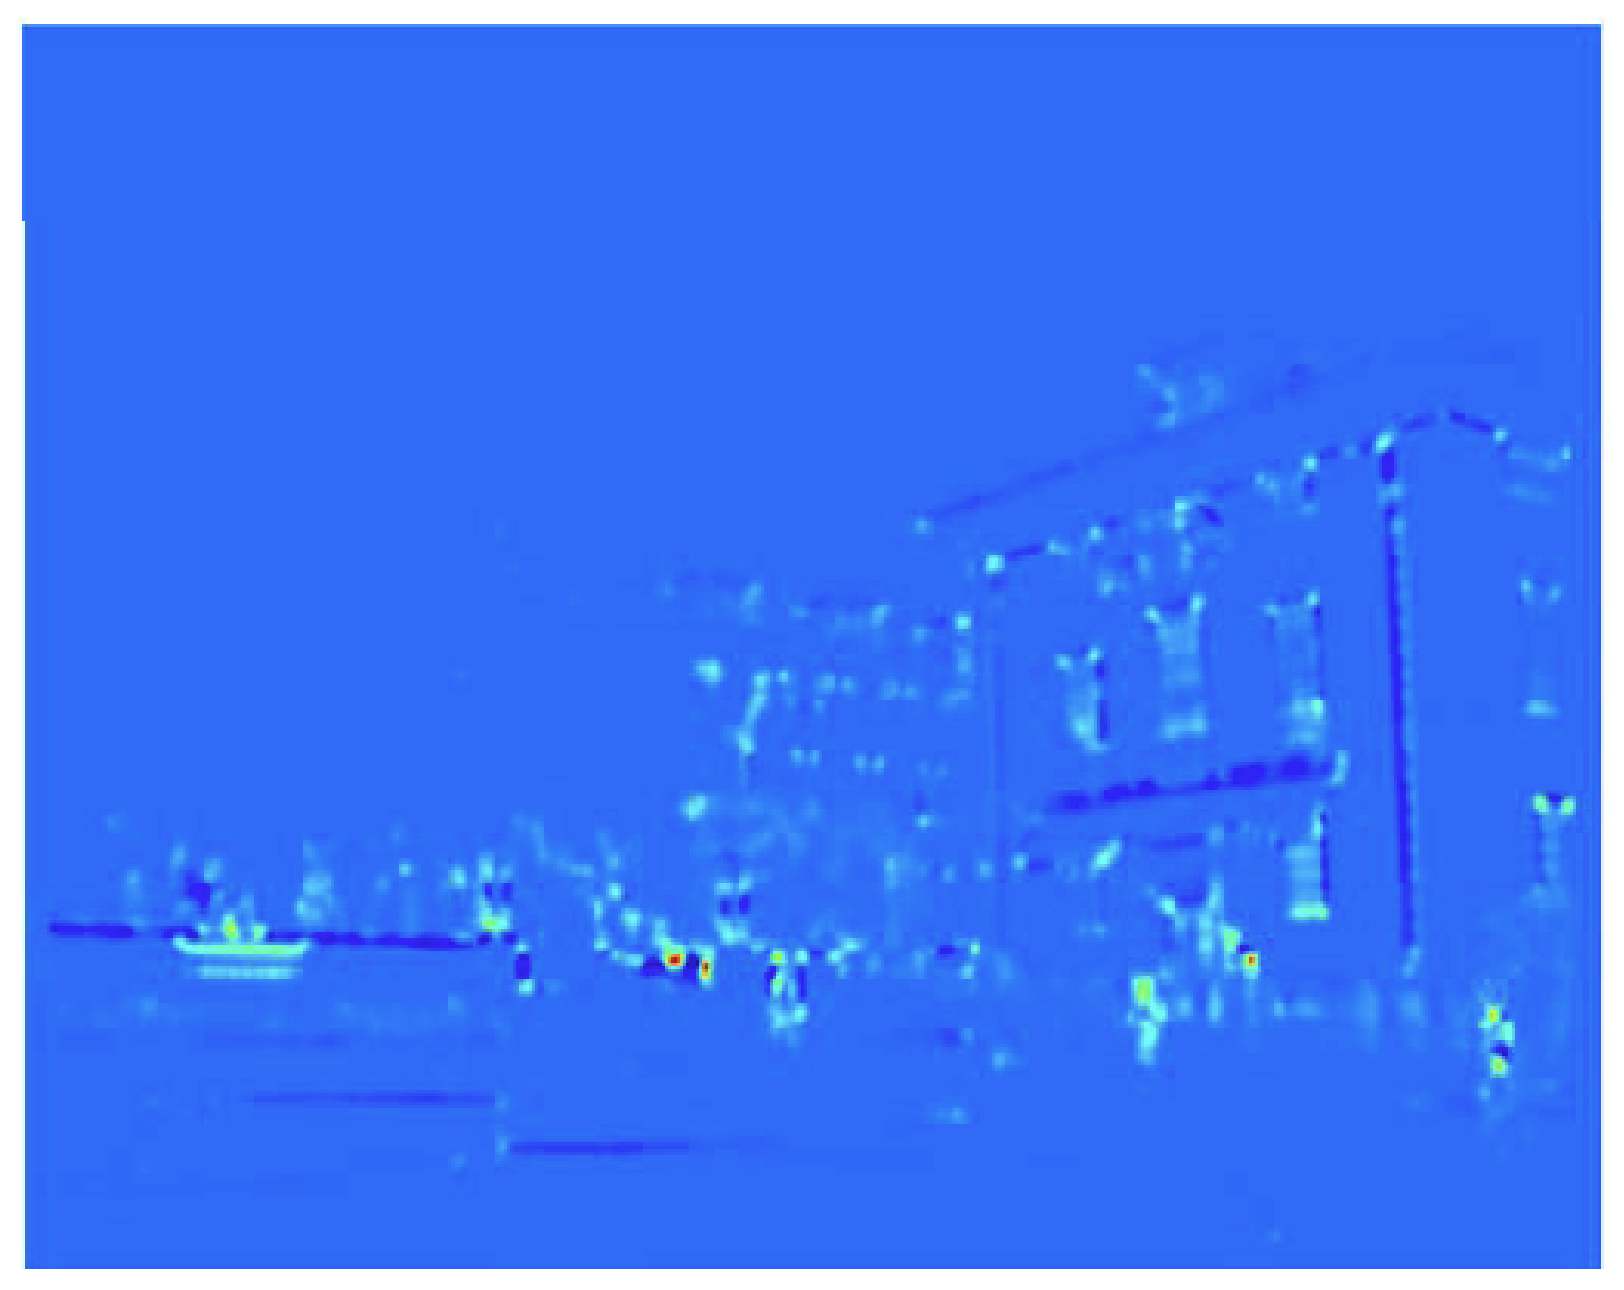
\includegraphics[width=0.6\textwidth]{img/cornernessheatmap.png}
    \caption{Search for parts of the image that have the most "cornerness"}
    \end{figure}
\end{frame}

\begin{frame}{Classical Feature Extraction}
    \begin{figure}
    \centering
    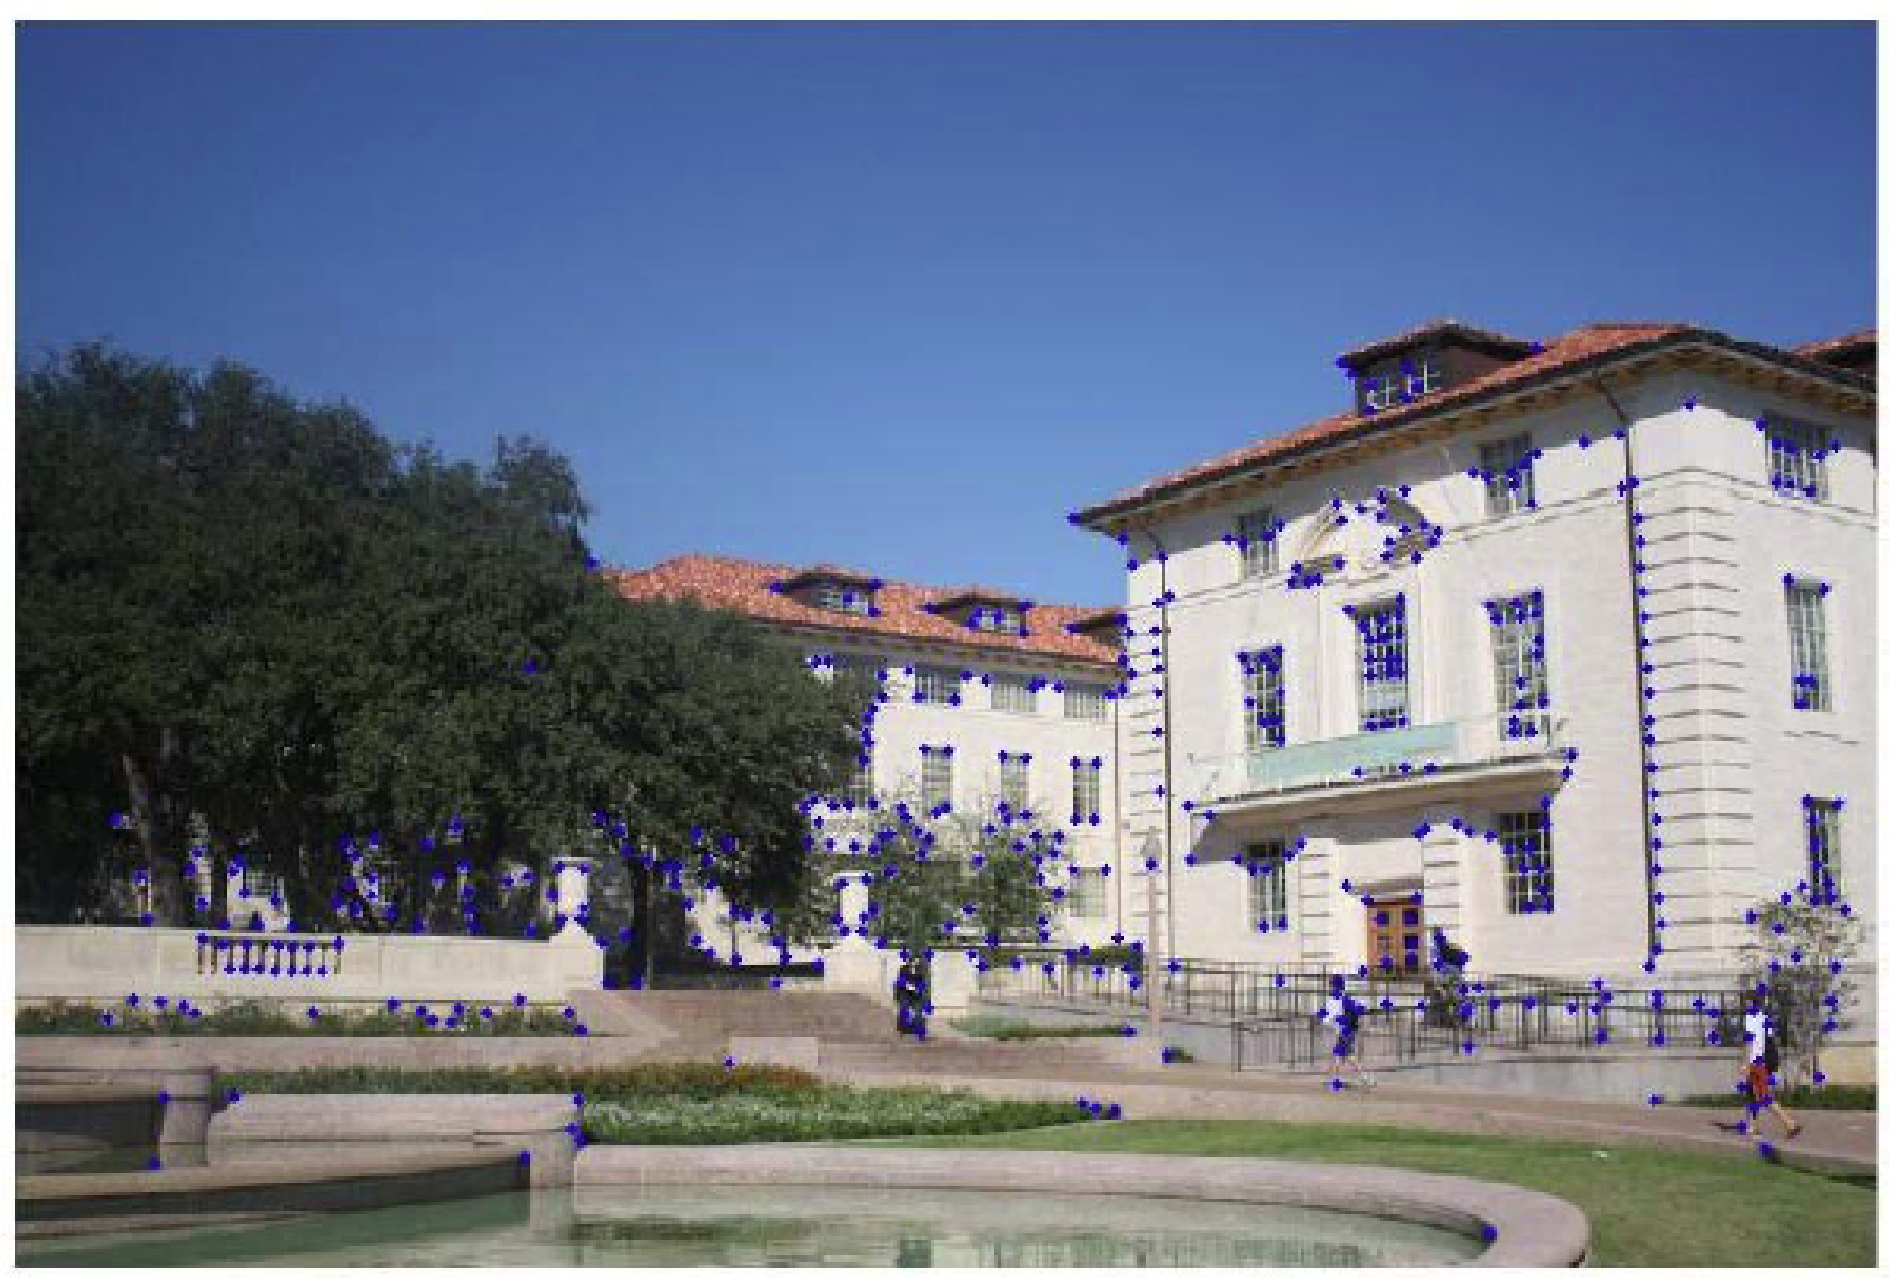
\includegraphics[width=0.8\textwidth]{img/houseinteresting.png}
    \caption{Based on our heatmap, extract points of interest}
    \end{figure}
\end{frame}

\begin{frame}{Classical Feature Extraction}
    \begin{figure}
    \centering
    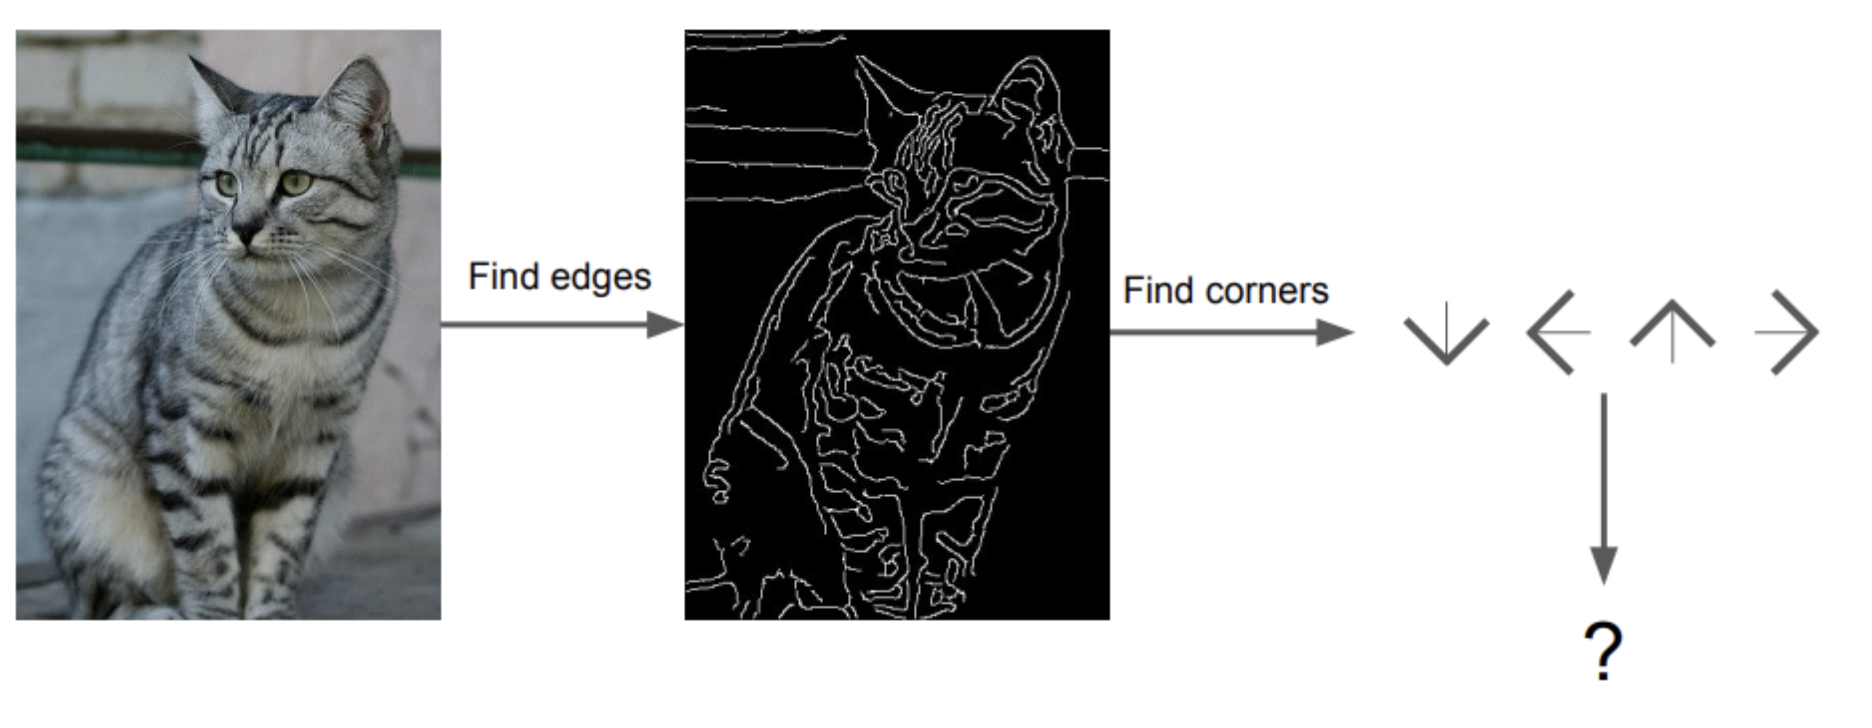
\includegraphics[width=0.8\textwidth]{img/edgecat.png}
    \caption{Extracting edges and corners can greatly reduce our input dimensionality while improving the model's understanding of local features}
    \end{figure}
\end{frame}

\section{Deep Convolutional Neural Networks}
\begin{frame}{Deep CNN}
\begin{itemize}
    \item Histograms and edges are called “shallow” features because we build them by hand
    \item We know we can learn neural network and linear model weights by \textbf{Gradient Descent}
    \item Can we also learn our features?
\end{itemize}
\end{frame}

\begin{frame}{Deep CNN}
\begin{figure}
    \centering
    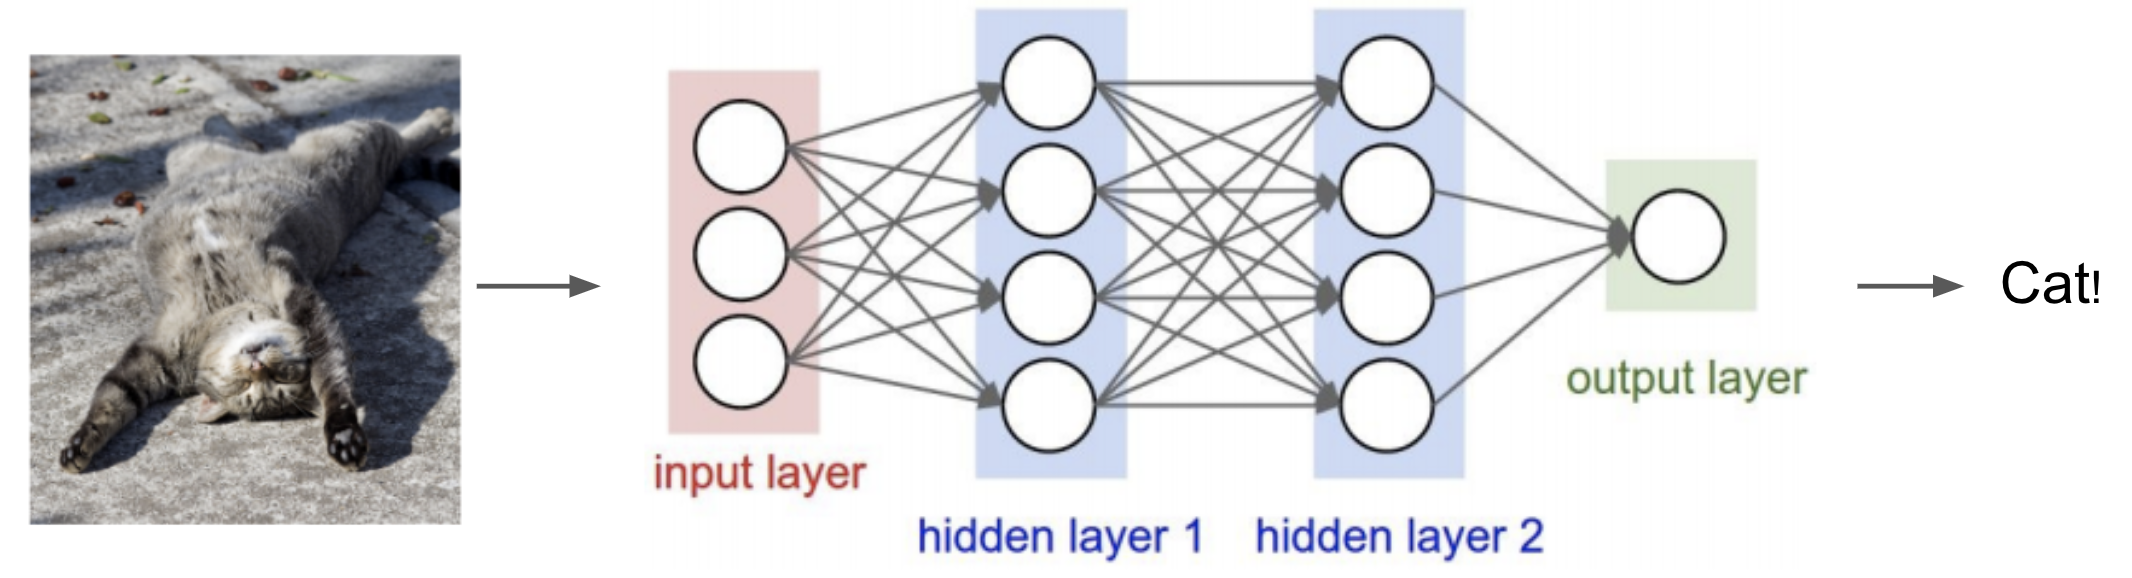
\includegraphics[width=1\textwidth]{img/catNN.png}
    \caption{Our neural network predicting cats must take either flattened cat or extracted features as input.}
\end{figure}
\end{frame}

\begin{frame}{Deep CNN}
\begin{figure}
    \centering
    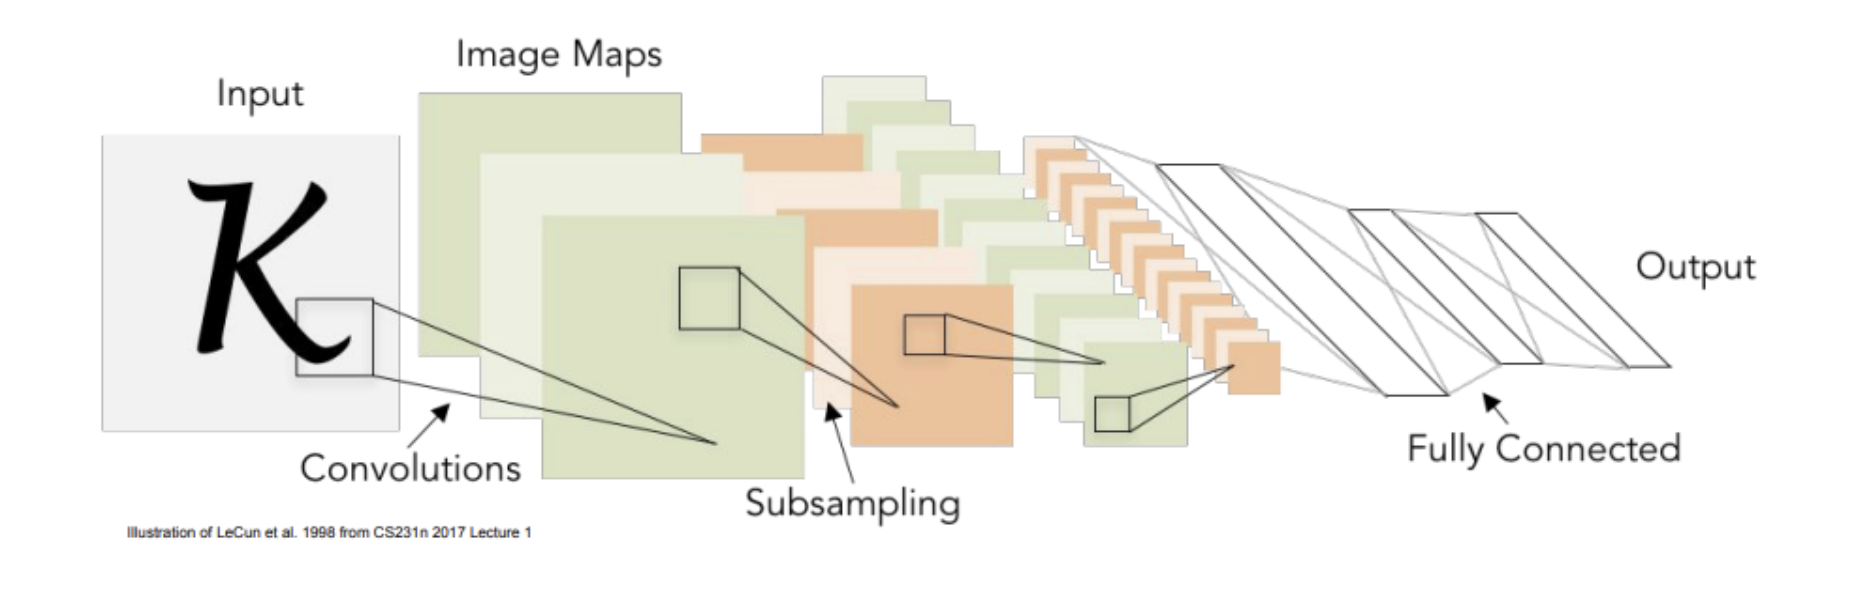
\includegraphics[width=1\textwidth]{img/dcnn.png}
    \caption{In modern Computer Vision, we rely on \textbf{Convolutional Neural Networks} to learn meaningful features by gradient descent.}
\end{figure}
\footnotetext{http://cs231n.stanford.edu/slides/2019/cs231n\_2019\_lecture05.pdf}
\end{frame}

\begin{frame}{Deep CNN}
\begin{figure}
    \centering
    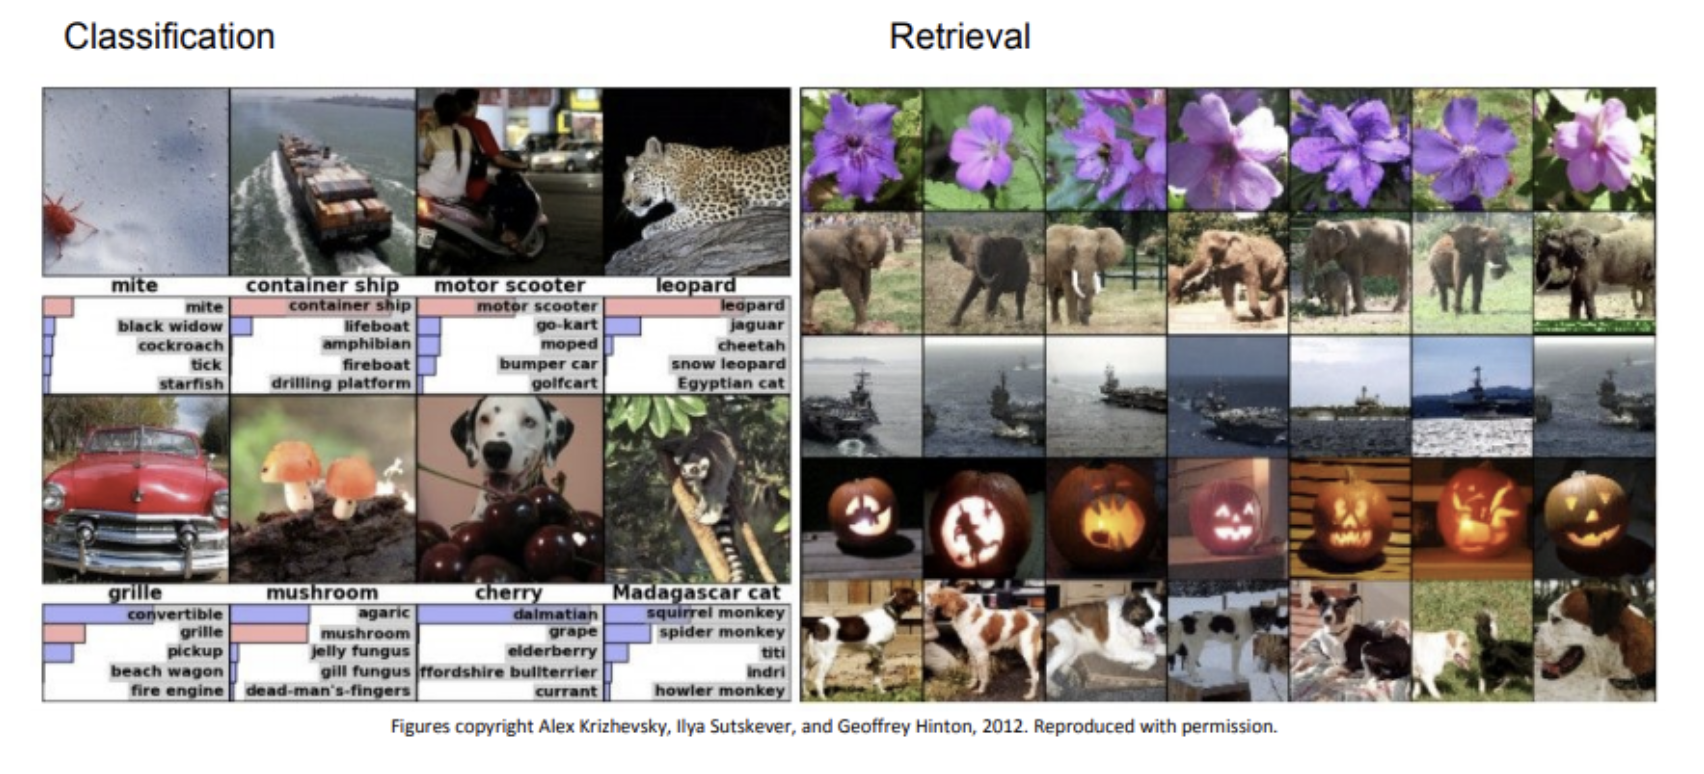
\includegraphics[width=1\textwidth]{img/cnnex1.png}
    \caption{Deep Convolutional Neural Networks are everywhere}
\end{figure}
\footnotetext{http://cs231n.stanford.edu/slides/2019/cs231n\_2019\_lecture05.pdf}

\end{frame}

\begin{frame}{Deep CNN}
\begin{figure}
    \centering
    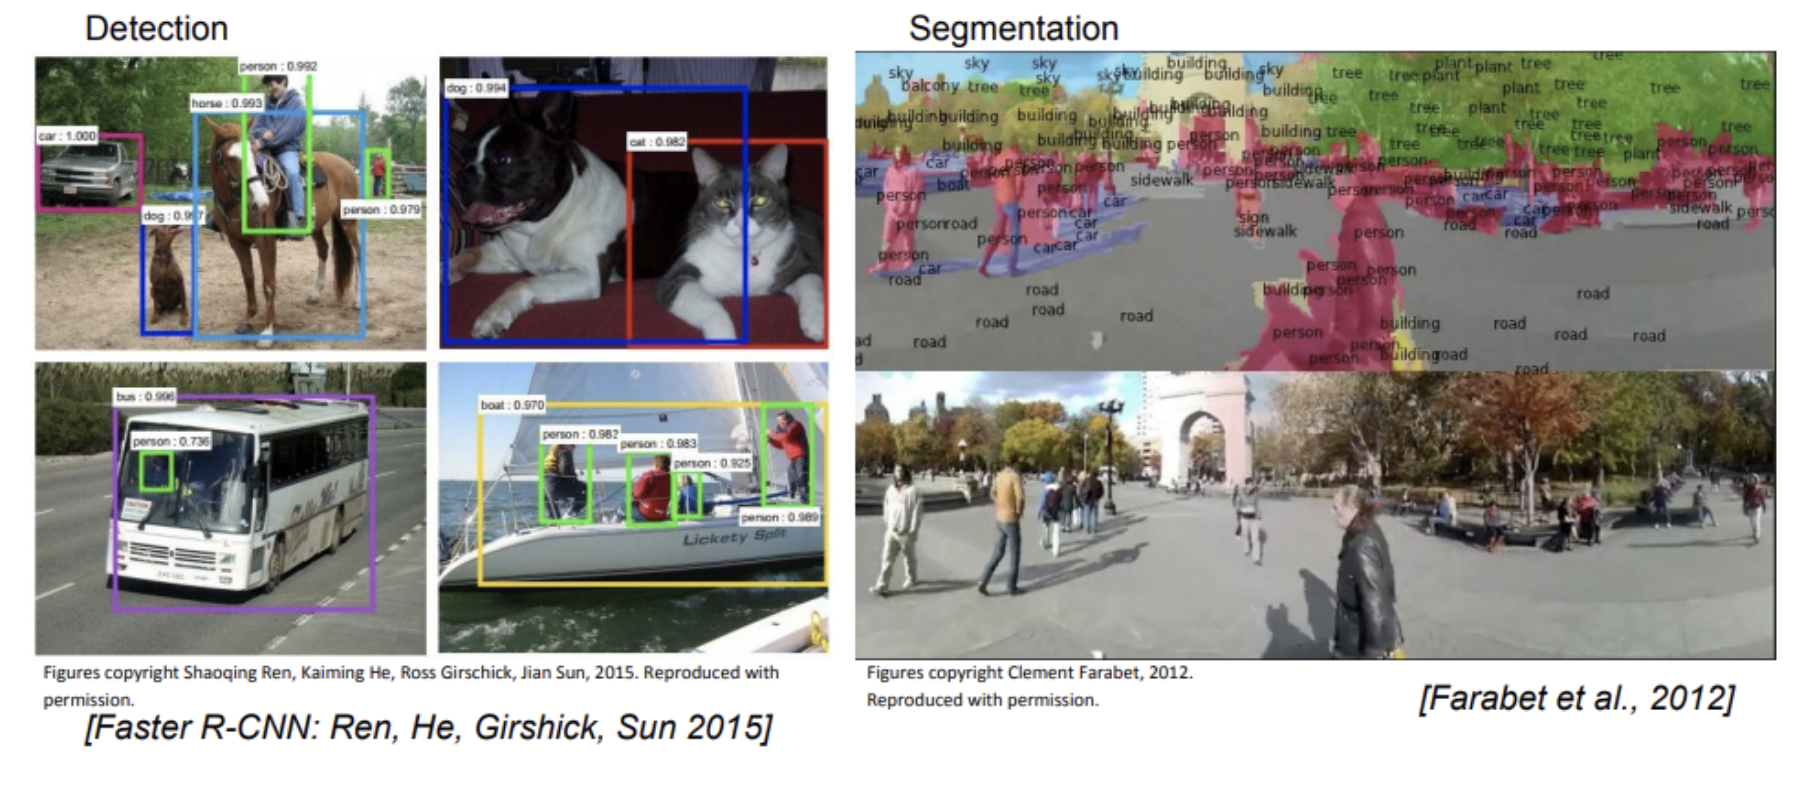
\includegraphics[width=1\textwidth]{img/cnnex2.png}
    \caption{Deep Convolutional Neural Networks are everywhere}
\end{figure}
\footnotetext{http://cs231n.stanford.edu/slides/2019/cs231n\_2019\_lecture05.pdf}
\end{frame}

\begin{frame}{Deep CNN}
\begin{figure}
    \centering
    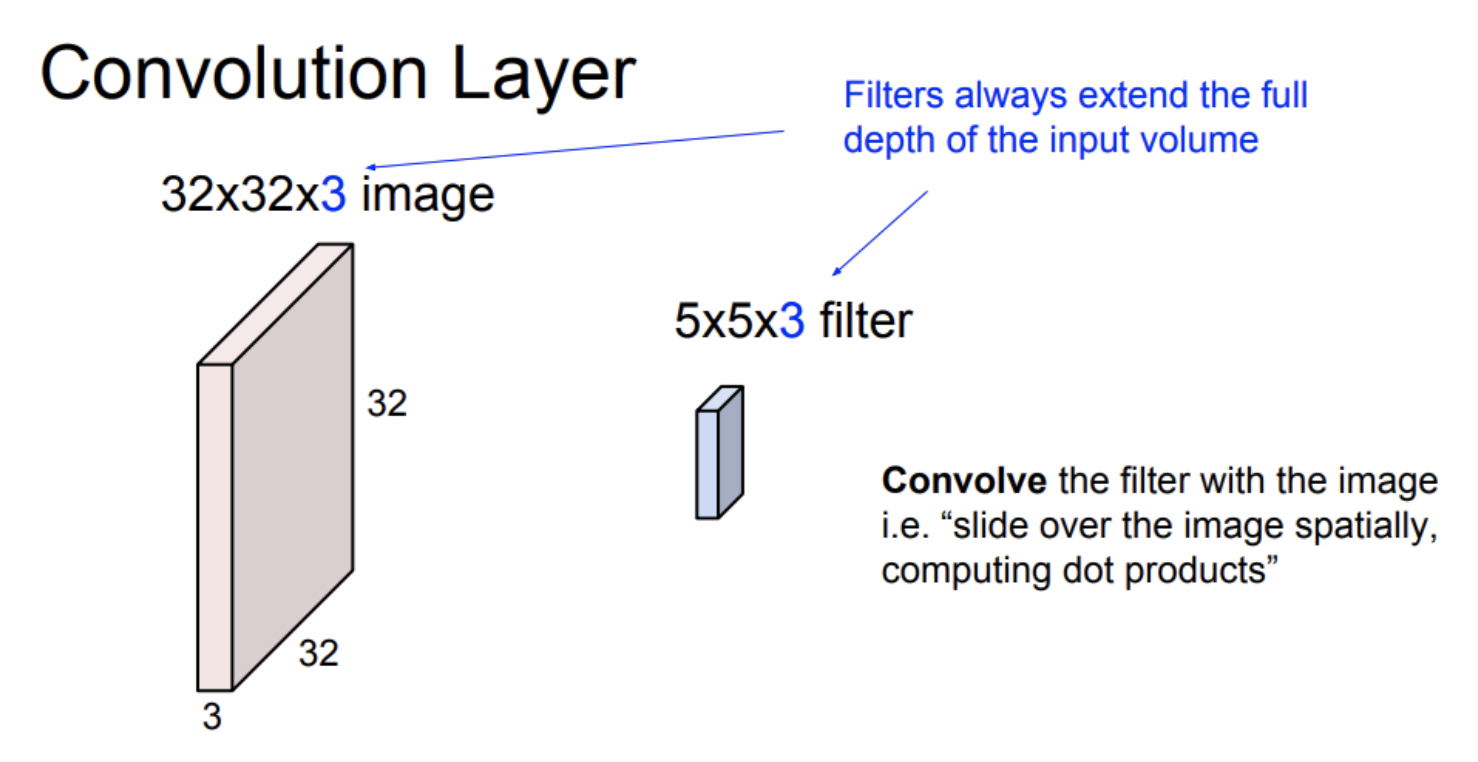
\includegraphics[width=0.8\textwidth]{img/convlayer1.png}
    \caption{Convolutional Layers}
\end{figure}
\footnotetext{http://cs231n.stanford.edu/slides/2019/cs231n\_2019\_lecture05.pdf}
\end{frame}

\begin{frame}{Deep CNN}
\begin{figure}
    \centering
    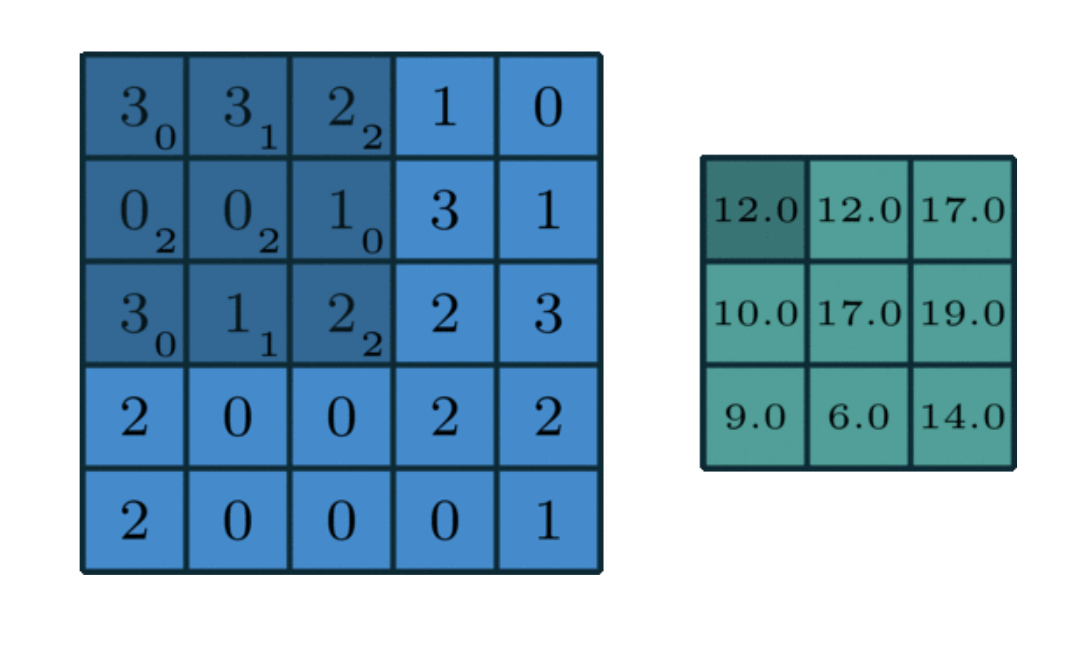
\includegraphics[width=0.8\textwidth]{img/convlayer2.png}
    \caption{Convolutional Layers}
\end{figure}
\end{frame}

\begin{frame}{Deep CNN}
\begin{figure}
    \centering
    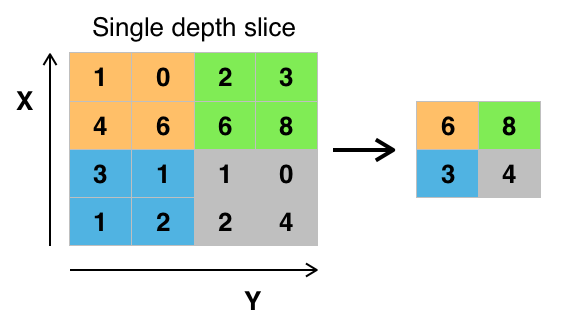
\includegraphics[width=0.8\textwidth]{img/Max_pooling.png}
    \caption{Max Pooling Layers}
\end{figure}
\end{frame}

\begin{frame}{Deep CNN}
\begin{figure}
    \centering
    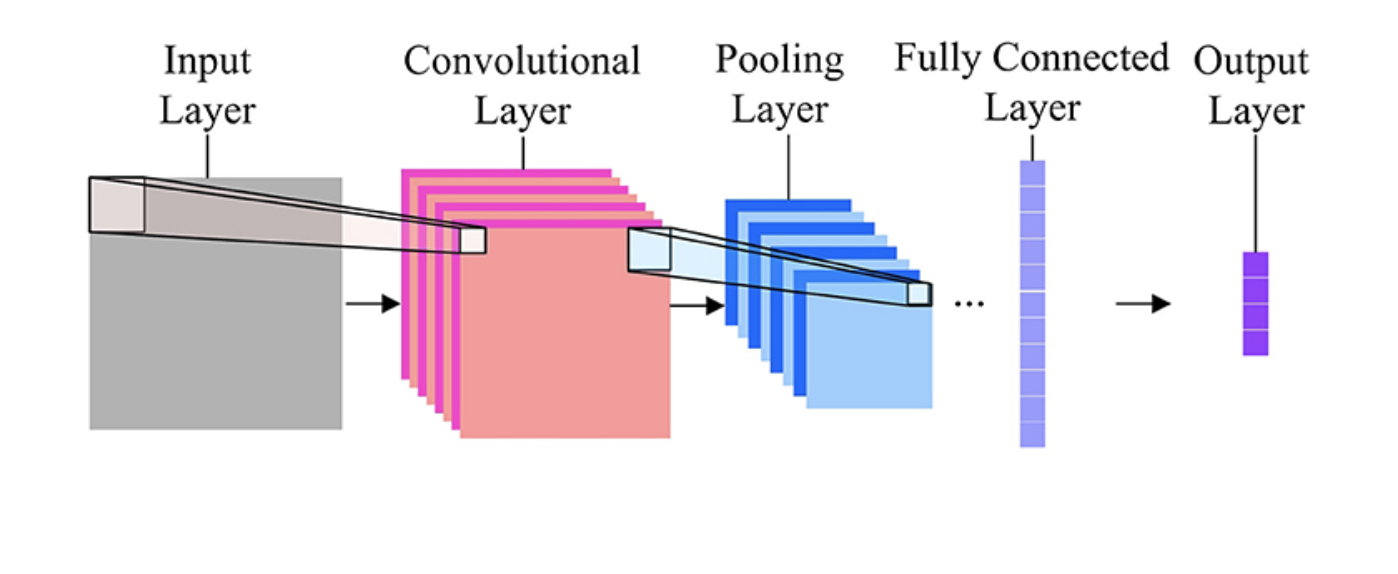
\includegraphics[width=1\textwidth]{img/cnn_structure.png}
    \caption{Full CNN Structure}
\end{figure}
\end{frame}

%%%%%%%% repeat first slide %%%%%%%%
\begin{frame}
\titlepage 
\end{frame}
\end{document}